\documentclass{scrartcl}

\usepackage{helvet}
\usepackage[T1]{fontenc}
\usepackage[ngerman]{babel}
\usepackage[utf8]{inputenc}
\inputencoding{utf8}
\usepackage{hyperref}
\usepackage{mathtools}
\usepackage[xindy,toc,section,acronym]{glossaries}
\makeglossaries
\usepackage[xindy]{imakeidx}
\makeindex
\usepackage{enumitem}
\usepackage{graphicx}
\usepackage{cleveref}
\usepackage[autostyle=true,german=quotes]{csquotes}
\renewcommand{\familydefault}{\sfdefault}
%----------------------------------
% thomi fa list implementation
%----------------------------------

\newlist{falist}{enumerate}{2}
\setlist[falist,1]{label={/FA\arabic{falisti}\arabic{falistii}/},align=left,labelwidth=17pt,labelsep=3pt,leftmargin=20pt}
\setlist[falist,2]{label={/FA\arabic{falisti}\arabic{falistii}/}}%,align=left,labelwidth=17pt,labelsep=3pt,leftmargin=0pt}

\usepackage{chngcntr}
\counterwithin{falistii}{falisti}

\newlist{pdlist}{enumerate}{2}
\setlist[pdlist,1]{label={/PD\arabic{pdlisti}\arabic{pdlistii}/},align=left,labelwidth=17pt,labelsep=3pt,leftmargin=20pt}
\setlist[pdlist,2]{label={/PD\arabic{pdlisti}\arabic{pdlistii}/}}%,align=left,labelwidth=17pt,labelsep=3pt,leftmargin=0pt}
\counterwithin{pdlistii}{pdlisti}

\newlist{nflist}{enumerate}{2}
\setlist[nflist,1]{label={/NF\arabic{nflisti}\arabic{nflistii}/},align=left,labelwidth=17pt,labelsep=3pt,leftmargin=20pt}
\setlist[nflist,2]{label={/NF\arabic{nflisti}\arabic{nflistii}/}}%,align=left,labelwidth=17pt,labelsep=3pt,leftmargin=0pt}
\counterwithin{nflistii}{nflisti}

\newlist{telist}{enumerate}{2}
\setlist[telist,1]{label={/T\arabic{telisti}\arabic{telistii}/},align=left,labelwidth=17pt,labelsep=3pt,leftmargin=20pt}
\setlist[telist,2]{label={/T\arabic{telisti}\arabic{telistii}/}}%,align=left,labelwidth=17pt,labelsep=3pt,leftmargin=0pt}
\counterwithin{telistii}{telisti}

\loadglsentries[main]{glossar}

\begin{document}


\title{Pflichtenheft: Lambda - Das Spiel, \\ Die Entwickler}
\author{Luca Becker, Henrike Hardt,\\Larissa Schmid, Adrian Schulte,\\Maik Wiesner}
\date{1. Dezember 2014}
\maketitle

\includegraphics[width=\textwidth]{assets/Lambdolino}
\thispagestyle{empty}

\clearpage

\thispagestyle{empty}
\tableofcontents
\thispagestyle{empty}

\clearpage
\setcounter{page}{1}




    

% ---------------
% Einleitung
% ---------------

\section{Einleitung}

Der derzeitige und auch kommende Ingenieursmangel in Deutschland ist
schon seit Langem Thema in den Medien. „Auf jeden Bewerber kommen
etwa 4 freie Stellen“%
\footnote{http://www.ingenieurwesen-studieeren.de/ingenieurmangel/, aufgerufen am 04.11.14%
}, „jeder zweite angehende Ingenieur bricht sein Studium ab“%
\footnote{http://www.zeit.de/studium/hochschule/2013-10/ingenieure-unis-fachkraeftemangel, aufgerufen am 04.11.14%
}, all diese Nachrichten geben Grund zur Sorge in Hinblick auf Deutschland
als Technologiestandort. Unsere Volkswirtschaft beruht nicht mehr
auf Wertschöpfung aus dem ersten und zweiten, sondern vor allem aus
dem dritten Sektor – damit dies weiterhin funktionieren kann, werden
vor allem Ingenieure benötigt. Doch an dem derzeitigen Mangel ist
nicht nur die Überalterung unserer Gesellschaft schuld, sondern vor
allem auch die fehlende Begeisterung von Jugendlichen für die sogenannten
MINT-Fächer (Mathematik, Informatik, Naturwissenschaft, Technik).
Um Deutschland als Standort auch weiterhin wettbewerbsfähig zu halten,
ist es somit wichtig, Kinder schon frühestmöglich spielerisch an Fragestellungen
aus diesen Bereichen heranzuführen. 

In der Informatik ist der Lambda-Kalkül ein wichtiges Konstrukt, der
zum Beispiel die Entwicklung funktionaler Programmiersprachen wesentlich
beeinflusst hat. Obwohl er damit eine große Bedeutung hat und sehr
mächtig ist in Bezug auf sowohl die Theoretische Informatik als auch
funktionale Programmierung, so sind die grundlegenden Regeln dennoch
nicht allzu komplex und leicht verständlich. 

Um Kindern also schon im Grundschulalter eine erste Auseinandersetzung
mit Themen der Informatik und damit auch der Ingenieurswissenschaften
zu bieten, eignet sich der Kalkül also sehr gut. Unsere nachfolgend
dargelegte Visualisierung der Funktionsweise des Kalküls mithilfe
von einfachen Formen und sie ineinander umwandelnden Maschinen ist
dabei besonders kindgerecht, wodurch der Kalkül anhand von einfachen
Lambda-Ausdrücken einfacher verstanden und verinnerlicht werden kann.
Diese Idee soll nun als \gls{gls:androidapp} umgesetzt werden, sodass Kinder
selbständig spielen können, der Fortschritt im Spiel aber auch jederzeit
durch Eltern oder Lehrkräfte einsehbar ist. 

\clearpage








% ---------------
% Zielbestimmungen
% ---------------

\section{Zielbestimmungen}


Die Kinder sollen durch das Spiel in die Lage versetzt werden, sich die Prinzipien des \gls{gls:lambdakalkuel}s spielerisch zu erarbeiten, ohne über Vorkenntnisse zu verfügen.

\subsection{Musskriterien}

\begin{enumerate}
	\item \label{muss:vermittelnlamba}Spielerisches Vermitteln des Lambda-Kalküls für Kinder ab acht Jahren
	\item \label{muss:simulationandroid}Das Spiel muss in der \gls{gls:simulationsumgebung} von \gls{gls:android} laufen
	\item \label{muss:touchinterface}komplett über das simulierte \gls{gls:touchinterface} bedienbar sein
	\item \label{muss:mvc}eine modulare Architektur besitzen (z.B. \gls{gls:mvc}-Prinzip)
	\item \label{muss:5indilevel}mindestens fünf individuelle \gls{gls:level}
	\item \label{muss:tutorial}\gls{gls:tutorial}-Level
\end{enumerate}

\subsection{Wunschkriterien}
Wunschkriterien seien von nun an im restlichen Pflichtenheft mit einem * markiert.

\begin{enumerate}
	\item \label{wunsch:werkstatt}Werkstatt zum Umbauen von Maschinen
	\item \label{wunsch:highscore}Highscore-Tabelle
	\item \label{wunsch:challengemode}Challengemode mit Zeitdruck
	\item \label{wunsch:multilang}Auslieferung in mehreren Sprachen
	\item \label{wunsch:8bit}Pixelgrafik / Retrolook / reduzierter Farbraum
	\item \label{wunsch:multiplechar}Mehrere Spielcharaktere (männlich, weiblich)
	\item \label{wunsch:multiplemode}Mehrere Spielmodi (siehe Aufgabentypen \ref{subsection:Aufgabentypen})
    \item \label{wunsch:story}Begleitende Story (siehe Handlung des Spieles \ref{subsection:Story})
    \item \label{wunsch:erweiterndeLevelelemente}Erweiternde Spielelemente und Levelelmente, z.B. Leitern, Wasserebenen, Leben, Rechts- und Linkshänder-Modi usw.
    \item \label{wunsch:wischgesten} Steuerung durch Wischgesten anstelle von Steuerkreuzen (wählbar durch Benutzer)
\end{enumerate}

\subsection{Abgrenzungskriterien}

\begin{enumerate}
	\item \label{abgrenz:online}Kein \gls{gls:onlinemodus} Modus
	\item \label{abgrenz:multiplayer}Keine Online-Anbindung
	\item \label{abgrenz:emu}Keine vorgesehene Kompatibilität mit anderen Geräten/Betriebssystemen ohne Emulation
\end{enumerate}

\clearpage










% ---------------
% Spielaufbau
% ---------------

\section{Spielaufbau}

\subsection{Spielprinzip}
Das Spielprinzip beruht auf dem Bewegen von Blöcken, indem der \gls{gls:anwender} die Blöcke hochhebt und wieder absetzt. Der \gls{gls:anwender} muss die verschiedenen Elemente des Spieles, die Maschinen, die Maschinen-Cluster und die Metallstücke, in den dafür vorgesehenen Ablagen positionieren. Hat er alle Elemente in die jeweils richtige Ablage gesetzt, erfolgt die Auswertung, anschließend öffnet sich die Tür zum nächsten \gls{gls:level}.

\subsection{Handlung des Spiels*} \label{subsection:Story}
Lambdor, der Vollstrecker, hat die Spielfigur entführt und in ein Haus mit vielen magischen Räumen gesperrt, deren Türen verschlossen sind. Um entkommen zu können, muss die Spielfigur die Türen öffnen. Dafür braucht sie besondere Metallstücke, diese hat Lambdor jedoch zerstört. Die Spielfigur kann sie wieder herstellen, dafür muss sie zunächst die Maschinen zusammenbauen, mit denen die Metallstücke hergestellt werden können. Glücklicherweise hilft Lambdalino, der kleine Bruder von Lambdor, der Spielfigur dabei. Er zeigt ihr, wie sie die Maschinen zusammenbauen muss und wie sie die Metallstücke herstellen kann. So kann die Spielfigur es schaffen, aus dem Wirrwarr der Räume zu entkommen.


\subsection{Spielelemente}

Zu Beginn eines \glspl{gls:level} wird die Spielfigur angezeigt. Diese bewegt sich zweidimensional durch die Welt und wird vom \gls{gls:spieler} gesteuert.

\begin{description}
	\item[Spielfigur] bewegt sich durch die Welt, sammelt Gegenstände, um mit diesen die Levelquest zu lösen
	\item[Leben*] Jeder \gls{gls:anwender} hat je \gls{gls:level} drei Leben, die er verlieren kann, z.B. wenn er ins Wasser fällt
	\item[Spielwelt] zweidimensionale Spielwelt auf einem Raster basierend, in der sich die Spielfigur bewegt
	\item[Spielebenen] verschiedene Ebenen in der Spielwelt, auf die, die Spielfigur springen kann. Sie sind auf einem Raster angeordnet:
		\begin{enumerate}[label=\arabic*]
			\item Landebenen: Auf diesen Ebenen liegen die Sammelgegenstände
			\item Wasserebenen*: Fällt die Spielfigur in das Wasser, muss er wieder am linken unteren Rand anfangen und er verliert ein Leben. Hat er kein Leben mehr, so muss er das \gls{gls:level} neu beginnen
		\end{enumerate}
	\item[Sammelgegenstände] \label{elemente:collectable}sind in der Spielwelt verteilt und müssen von der Spielfigur eingesammelt werden, um in den Ablagen platziert zu werden. Diese bestehen aus:
	\begin{enumerate}[label=\arabic*]
		\item Maschinen (entspricht der Abstraktion)
		\item Metallstücke (entspricht der Variablen)
		\item Maschinen-Cluster (entspricht der Applikation)
	\end{enumerate}
	\item[Ablage] sind die markierten Stellen, an denen Spielobjekte abgelegt werden können
	\item[Levelquest] sind gegebene Aufgaben, die zum Abschließen des Levels erfüllt werden müssen
	\item[Leveltür] bildet den Abschluss eines Levels. Sobald alle Quests in dem \gls{gls:level} gelöst wurden, wird die Tür freigeschaltet
\end{description}

\subsection{Regeln}

\begin{description}

\begin{minipage}{1\textwidth}
	\item[Spielregeln] \label{spielaufbau:Spielregeln} 
	Die Spielfigur beginnt an der unteren, linken Ecke der Spielwelt und muss es schaffen die Tür an der rechten unteren Ecke zu öffnen. Dies gelingt, indem diverse Objekte (Maschinen, Metallobjekte und Maschinen-Cluster) auf dem Spielfeld in Position gebracht werden, sodass diese nach den Prinzipien des Lambda-Kalküls einen Lambda-Ausdruck bilden, welcher zum gewünschten Ergebnis zusammengefasst oder gelöst werden kann.\\
	Die Spielfigur muss neben einem Objekt stehen, um dieses aufheben zu können.\\
	Der Spielfigur kann immer nur ein Objekt tragen. Um ein anderes Objekt aufzuheben muss er erst das Objekt, das er trägt, ablegen.\\
	Um auf die oberen Ebenen der Spielwelt zu gelangen, kann die Spielfigur springen, dabei ist zu beachten, dass die Figur nur eine feste Höhe hochspringen kann und der \gls{gls:anwender} somit auf Ebenen außerhalb seiner Reichweite nicht durch einfaches Springen gelangen kann. Die Figur kann auch springen, wenn sie etwas in den Händen trägt (dabei kann es zu einer geringen Trägheit kommen, z.B. ungenauere Spielsteuerung (diese ist gewollt und soll das Spiel ein wenig schwieriger gestalten))*.\\
	Befindet sich in jeder freien Ablage ein Objekt, wird der daraus resultierende Lambda-Ausdruck ausgewertet. Falls die Maschinen und Metallstücke in den richtigen Ablagen liegen und der $\lambda$-Kalkül erfüllt ist, wird dem \gls{gls:anwender} das Ergebnis und die spezifische Abarbeitung des Maschinenkonstrukts nach den Regeln des $\lambda$-Kalküls gezeigt. Anschließend öffnet sich die Tür am Level-Ende. Das \gls{gls:level} gilt als geschafft, sobald diese erreicht ist.\\
	
\end{minipage}

\begin{minipage}{1\textwidth}
	\item[Die Verarbeitungsregel der Maschinen] Die Verarbeitung der einzelnen Objekte erfolgt in fester Reihenfolge.\\
	Es wird immer nur ein Objekt zu einem bestimmten Zeitpunkt verarbeitet.\\
	Wie das Objekt verarbeitet wird, bestimmt die jeweilige Maschine.\\
	Was die Maschine verarbeiten soll, befindet sich immer rechts neben dieser Maschine.\\
	Die Maschinen werden in fester Reihenfolge angeordnet und verarbeiten nacheinander die gegebenen Objekte.\\
	Dabei kann jede Maschine nur einmal etwas verarbeiten, nach der Verarbeitung verschwindet sie.\\
	Jede Maschine kann die Anzahl des zu verarbeitenden Objekts und ggf. dessen Farbe/Muster verändern. Hierbei ist zu beachten, dass eine Maschine auch ein Objekt komplett entfernen kann. Was eine Maschine genau am zu verarbeitenden Objekt verändert, ist durch ihr Aussehen eindeutig bestimmt.\\
	Das verarbeitete Objekt landet im Bereich oberhalb der Maschine an vorgegebenen Stellen, die durch Metallobjekte, die dieselbe Farbe wie die Maschine besitzen, gekennzeichnet werden (Die Maschine verarbeitet quasi diese gleichfarbigen Blöcke zu Duplikaten des Input-Objekts).\\
	Nachdem die Maschine verschwunden ist, rücken die Objekte über ihr alle um eine Position nach unten und die in der untersten Ebene am weitesten links liegende Maschine beginnt die Verarbeitung.\\
\end{minipage}	
	
\begin{minipage}{1\textwidth}
	\item[Sonderfälle/regeln:] Maschinencluster: Ein Maschinencluster ist eine besondere Form der Anordnung von Maschinen, er verarbeitet keinen Input, sondern dient als eine Art \enquote{Klammerung}. Ist ein Maschinencluster an der Reihe zu arbeiten, so werden alle Objekte in diesem Cluster nach den normalen Verarbeitungsregeln zuerst verarbeitet, bis nur noch eine Maschine und eine Menge an Metallobjekten darin vorhanden sind. Danach verschwindet der Cluster und sein Inhalt übernimmt seinen Platz in der aktuellen Verarbeitung.\\
	$\alpha$-Regel: Diese Regel besagt, dass, falls eine Maschine eine andere Maschine oder ein anderes Metallobjekt verarbeitet, jedoch oberhalb (in der Verschachtelung) der arbeitenden Maschine bereits mindestens ein Objekt der selben Farbe wie das Input-Objekt vorhanden ist, das Input-Objekt und alle dazugehörigen Objekte eine andere Farbe, die noch nicht vergeben ist, erhalten.\\
\end{minipage}

\end{description}

\subsection{Steuerung}  \label{subsection:Steuerung}

Zur Steuerung der Spielfigur in den einzelnen Levels werden im unteren Teil des Bildschirms insgesamt 5 Buttons eingeblendet, die sich in 2 Gruppen aufteilen.\\
Die Positionierung dieser Buttons kann profilspezifisch geändert werden, dabei gibt es jedoch nur 2 Wahlmöglichkeiten*.\\

\begin{enumerate}
	\begin{minipage}{1\textwidth}
			\item Gruppe 1:\\
			Die erste Gruppe an Buttons besteht aus zwei Buttons, durch welche der \gls{gls:anwender} die Spielfigur nach Rechts und Links bewegen kann.\\
			Die Spielfigur bewegt sich dabei solange in die jeweilige Richtung, wie der \gls{gls:anwender} den Button drückt.\\
			Diese Button-Gruppe ist standardmäßig in der linken unteren Ecke des Bildschirms.\\
			Der \gls{gls:anwender} kann immer nur einen der beiden Buttons, nie beide zur selben Zeit drücken.\\
	\end{minipage}
	
	\begin{minipage}{1\textwidth}
			\item Gruppe 2:\\
			Die zweite Gruppe an Buttons besteht aus drei Buttons, diese dienen zum Einen der Interaktion der Spielfigur mit den Spielobjekten, die es platzieren muss, und zum Anderen der Funktion des Springens und Duckens* der Spielfigur.\\
			Der Button zur Interaktion mit den Spielobjekten hat zwei Funktionen: Der \gls{gls:anwender} kann ein Spielobjekt, das in Blickrichtung direkt neben der Spielfigur liegt, aufheben (und trägt es somit), falls die Spielfigur bereits ein Objekt trägt, dieses in Blickrichtung in das benachbartes Feld ablegen. Diese Aktionen können nicht parallel zu einer der anderen drei Aktionen (Bewegen, Springen, Ducken) ausgeführt werden, die Spielfigur muss stehen.\\
			Der Springen-Button lässt die Spielfigur eine feste Höhe hochspringen, durch paralleles Drücken der Bewegungstasten kann zusätzlich ein Sprung nach links oder rechts ausgeführt werden. Andere Buttons können nicht parallel betätigt werden.\\
			Der Ducken-Button* lässt die Spielfigur sich ducken. Dies führt zu einer Verringerung ihrer Größe, was insbesondere, wenn sie ein Objekt trägt, hilfreich sein kann. Die Spielfigur kann sich parallel zum Ducken nur bewegen, nicht springen oder ein Objekt aufnehmen oder ablegen.\\
	\end{minipage}

	\item Im Folgenden sehen sie eine ungefähre Darstellung der Steuerung. Die Alternative, die profilspezifisch gewählt werden kann*, sieht eine Vertauschung der beiden Button-Gruppen vor, wobei die Button-Gruppe 2 zusätzlich gespiegelt wird.\\
	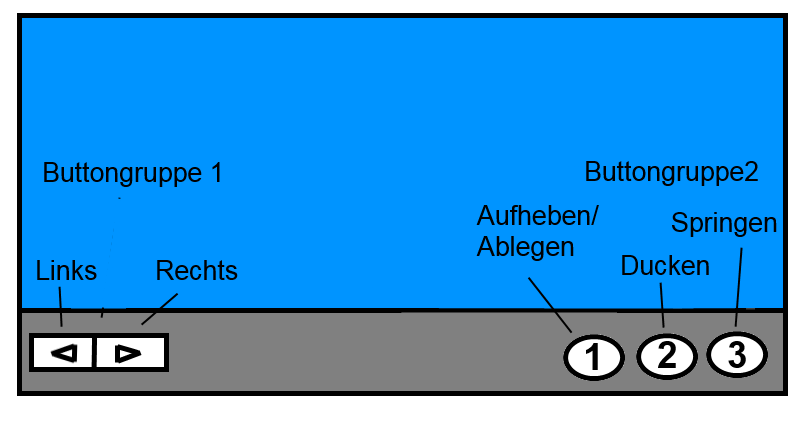
\includegraphics[scale=0.5]{assets/Steuerung}
\end{enumerate}


\subsection{Lambda-Kalkül}  \label{subsection:LambdaKalkül}
\label{LambdaKalkül:AlgemeineErklärung}

 Der $\lambda$-Kalkül ist eine formale Sprache, die im Allgemeinen dazu dient, Funktionen zu definieren bzw. beschreiben.\\
In unserem Fall beschränken wir uns jedoch auf die beiden grundlegenden Regeln des $\lambda$-Kalkül, die $\alpha$-Regel und die $\beta$-Regel. Das Spiel soll dem \gls{gls:anwender} diese beiden wichtigen Regeln des $\lambda$-Kalkül anschaulich erklären.

\subsubsection{\texorpdfstring{$\alpha$}{Alpha}-Konversion}

Die Alpha-Regel besagt im $\lambda$-Kalkül, dass die Variablen eines $\lambda$-Terms jederzeit umbenannt werden dürfen, um die Eindeutigkeit dieser Terme zu waren. Beispielsweise:
\[
	\lambda x.x [x \leftarrow y] \Rightarrow \lambda y.y.
\]

Wichtig ist hierbei, dass keine Doppelverwendung von Variablennamen in unterschiedlichen $\lambda$-Termen entsteht. Vielmehr ist diese Regel dazu gedacht, beim Auftreten einer Doppelbelegung eine der beiden Variablen umzutaufen, um eindeutige $\lambda$-Terme zu formen.

\subsubsection{\texorpdfstring{$\beta$}{Beta}-Reduktion}

Die $\beta$-Regel dient der Vereinfachung, Auflösung oder Umformung von $\lambda$-Termen.\\
Sie besagt, dass ein $\lambda$-Term, von zum Beispiel folgender Form:

\[
	(\lambda x.x+2)(z)
\]

umgeformt werden kann, indem der Ausdruck \enquote{$z$} in den Term hinter dem Punkt eingesetzt wird und zwar für genau die Variable, die zwischen \enquote{$\lambda$} und dem Punkt steht, um es anschaulich zu erklären. Beispielsweise:
\[
	(\lambda x.x+2)(z) = (x+2)[x \leftarrow z] = z + 2
\]
Wichtig ist, dass hierbei sowohl z als auch x für alles stehen können. Also kann x insbesondere auch eine Funktion sein und z zum Beispiel ein weiterer kompletter $\lambda$-Term.

\subsubsection{Beispiel für der \texorpdfstring{$\lambda$}{Lambda}-Kalkül}
\[
	\begin{aligned}
		\lambda f.f(f(2))(\lambda x.x+2)&\xRightarrow{\beta} (f(f(2)))[f \leftarrow \lambda x.x+2] \\
		&\xRightarrow{\beta} (\lambda x.x+2)((\lambda x.x+2)(2)) \\
		&\xRightarrow{\beta} (\lambda x.x+2)((x+2)[x \leftarrow 2]) \\
		&\xRightarrow{\beta} (\lambda x.x+2)(2 + 2) \\
		&\xRightarrow{\beta} (x+2)[x \leftarrow 2 + 2] \\
		&\xRightarrow{\beta} 2 + 2 + 2 = 6
	\end{aligned}
\]



\subsection{Levelaufbau}  \label{subsection:Levelaufbau}


\begin{description}
	
	\begin{minipage}{1\textwidth}
		\item[Tutorial:] \label{Levelaufbau:Tutorial}  Das \gls{gls:tutorial} umfasst die ersten \gls{gls:level} des Spiels. Der \gls{gls:anwender} soll hier das Spielprinzip im Spielmodus Puzzle Schritt für Schritt verstehen.
		Umgesetzt wird dies durch sehr einfache Level, wobei in jedem \gls{gls:level} ein neuer Faktor hinzukommt.\\
		Im ersten \gls{gls:level} liegt der Fokus darauf, dem \gls{gls:anwender} die Steuerung und die Level-Elemente zu erklären. 
		In den darauffolgenden Levels wird die Spielmechanik mit Maschinen und Metallobjekten erklärt.\\
		Zwischen den Levels wird die Story* eventuell durch kleine, animierte Zwischenszenen erklärt.\\		 
	\end{minipage}
		

	\item[Levelbeispiel:] \label{Levelaufbau:Levelbeispiel} Als Level-Beispiel dient das erste \gls{gls:tutorial}-Level. Es wird in mehrere Bilder aufgeteilt, um die möglichen Aktionen des \gls{gls:anwender} zu erklären, sowie den grundlegenden Ablauf eines Levels darzustellen.\\
	
	\begin{enumerate}
		\begin{minipage}{1\textwidth}
			\item \label{Levelaufbau:Levelstart	} Zum Level-Start befindet sich die Spielfigur am rechten Rand der Spielwelt,\\
			außerdem ist das Level-Ziel eingeblendet.\\
			Das Level-Ziel gibt die Zielkonstellation an, die das zusammengesetzte Konstrukt aus Maschinen und Metallobjekten nach Verarbeitung nach den Regeln des $\lambda$-Kalküls haben soll.\\
			Das Level-Ziel kann der \gls{gls:anwender} durch einen Klick auf den Hacken unten rechts ausblenden und sich jederzeit durch einen Klick auf den Button mit dem ``Fahnen-Symbol'' unten in der Mitte des Bildschirms anzeigen lassen.\\ Solange Hinweise oder das Level-Ziel eingeblendet sind, kann der \gls{gls:anwender} keine anderen Aktionen ausführen.\\
			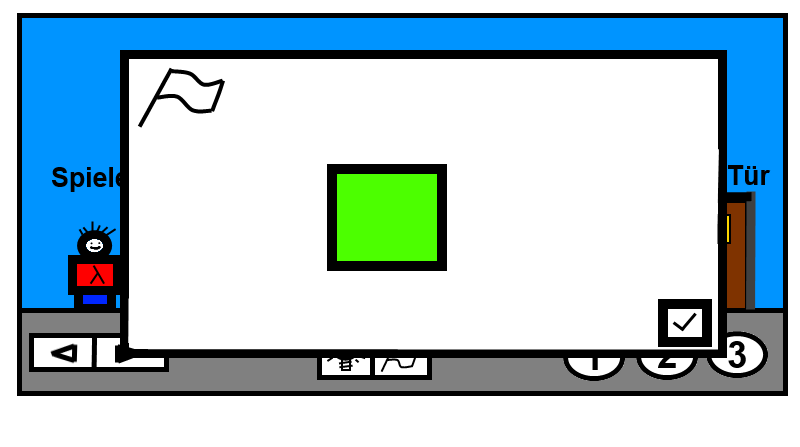
\includegraphics[scale=0.5]{assets/Levelziel}
		\end{minipage}
		
		\begin{minipage}{1\textwidth}
			\item \label{Levelaufbau:ErsteSchritte} Nach Ausblenden des Level-Ziels kann der \gls{gls:anwender} mit dem Lösen des Levels beginnen. Hierzu muss er die Spielfigur zum Metallobjekt bewegen, dieses per Button-Druck aufheben und anschließend in die freie Ablage daneben platzieren.\\
			Die über den Objekten angezeigten Namen dienen lediglich zur Erklärung, welches Objekt was darstellen soll und wird im eigentlichen Spiel nicht angezeigt.\\
			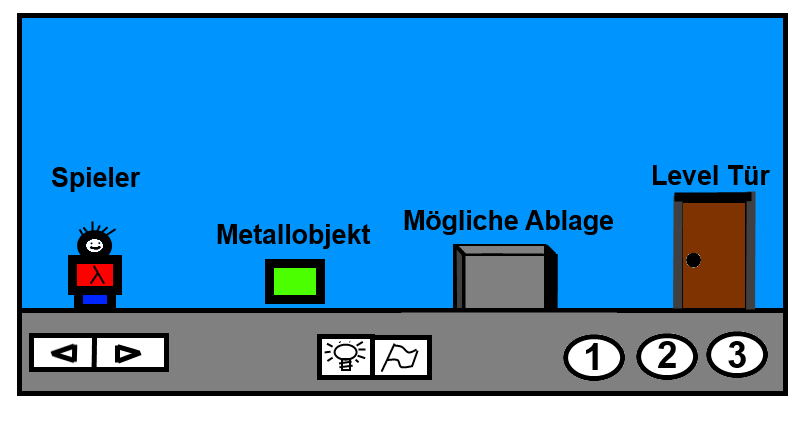
\includegraphics[scale=0.5]{assets/Level1mA}
		\end{minipage}
		
		\begin{minipage}{1\textwidth}
			\item \label{Levelaufbau:Levelende} Sind alle Ablagen gefüllt, so beginnt die Auswertung des Konstrukts.\\ Führt das Konstrukt zum gewünschten Ergebnis, so öffnet sich die Level-Tür  und der \gls{gls:anwender} kann durch Erreichen dieser Tür das \gls{gls:level} beenden. Dadurch gelangt er ins Auswertungsmenü.\\
			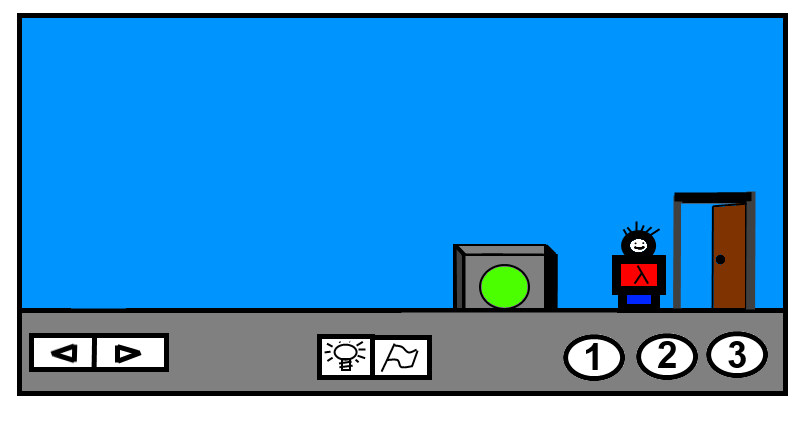
\includegraphics[scale=0.5]{assets/LevelEnde}
		\end{minipage}
		
		\begin{minipage}{1\textwidth}
			\item \label{Levelaufbau:Levelhinweis} Während des Spielens eines Levels kann der \gls{gls:anwender} jederzeit das Hinweisfenste*r öffnen. Dieses liefert, durch ein Bild dargestellt, levelspezifisch einen Hinweis auf die Zielkonfiguration des jeweiligen Levels.\\
			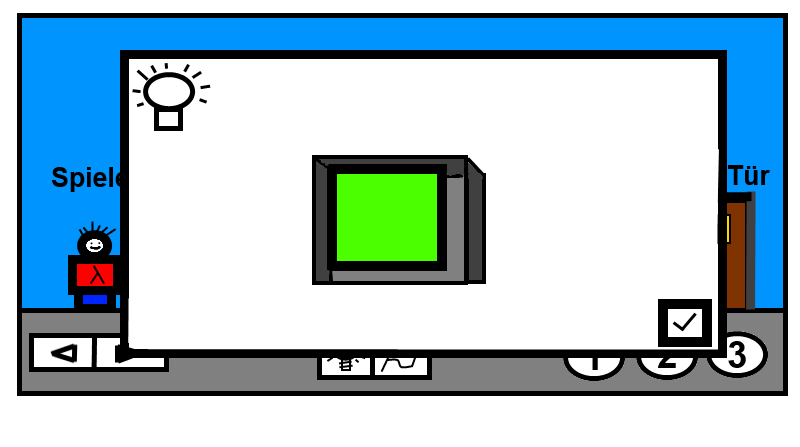
\includegraphics[scale=0.5]{assets/Levelhinweis}
		\end{minipage}
	\end{enumerate}
	
\clearpage

	\item[Konstrukte:] \label{Levelaufbau:Konstrukte} Im Folgenden sind einige Konstrukte, die in Leveln möglich sind, jeweils mit einer kurzen Erklärung aufgeführt.\\
	
		\begin{minipage}{1\textwidth}
			Einfacher Aufbau einer Maschine (grün) mit einem rechts daneben befindlichen Metallobjekt(Blau) als Input.\\
			In diesem Fall würde bei der Abarbeitung kein Ergebnis übrig bleiben, da die Maschine keine Metallobjekte besitzt, die es zu dem Input-Objekt verarbeiten könnte. Das heißt, das Resultat wäre nichts: sowohl das Metallobjekt als auch die Maschine verschwinden bei der Verarbeitung.\\
			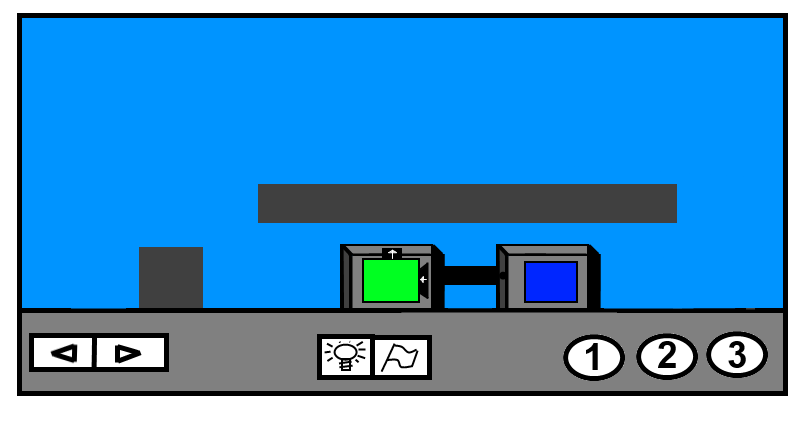
\includegraphics[scale=0.5]{assets/LevelBsp1}
		\end{minipage}
		
		\begin{minipage}{1\textwidth}
			Einfacher Aufbau einer Maschine (grün) mit einem zugehörigen Output-Metallobjekt (grün) darüber und einem rechts daneben befindlichen Metallobjekt (blau) als Input.\\
			In diesem Fall würde bei der Abarbeitung als Ergebnis ein blaues Metallobjekt übrig bleiben. Die Maschine würde ihr grünes Output-Objekt zu einem Duplikat des Input-Objekts verarbeiten, dabei verschwinden sowohl die Maschine als auch das Input-Objekt.\\
			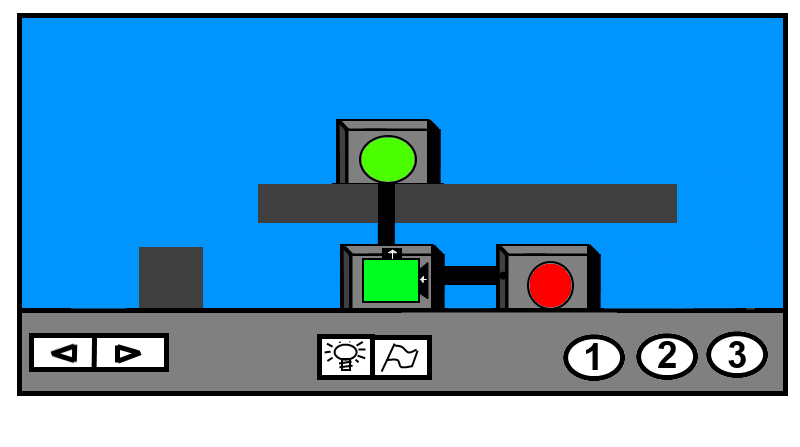
\includegraphics[scale=0.5]{assets/LevelBsp1Out}\\
		\end{minipage}
		
		\begin{minipage}{1\textwidth}
			Einfacher Aufbau einer Maschine (grün) mit zwei zugehörigen Output-Metallobjekten (grün) darüber und einem rechts daneben befindlichen Metallobjekt(Blau) als Input.\\
			In diesem Fall würden bei der Abarbeitung als Ergebnis zwei blaue Metallobjekte übrig bleiben. Die Maschine würde ihre grünen Output-Objekte zu Duplikaten des Input-Objekts verarbeiten. Dabei verschwinden sowohl die Maschine als auch das Input-Objekt.\\
			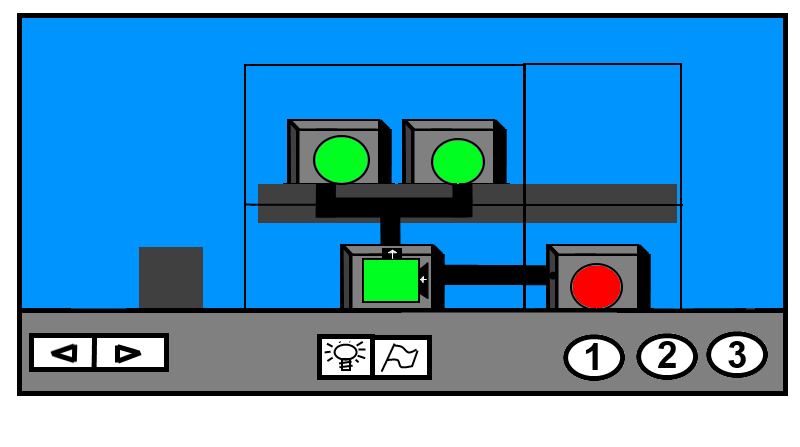
\includegraphics[scale=0.5]{assets/LevelBsp2Out}\\
		\end{minipage}
		
		\begin{minipage}{1\textwidth}
			Wie im oberen Bild zu erkennen ist, sind die Ablagen in eine Art Raster unterteilt.\\
			Dabei gilt, dass die unterste Ebene die primäre Verarbeitungsebene darstellt. Jede Maschine kann zusätzlich über sich eine Reihe von weiteren Ebenen haben, die eine Verschachtelung darstellen sollen. In dieser Verschachtelung können Metallobjekte der gleichen Farbe wie die darunterliegende Maschine sein, welche der Maschine als Output-Objekte, die sie bearbeiten soll, dienen, oder Metallobjekte anderer Farbe sowie weitere Maschinen mit dazugehörigen Verschachtelungsebenen. Welche Ablage zu welcher Ebene oder zu welcher Maschine gehört, wird durch geschickte Positionierung der Ablagen oder Verdeutlichung durch Röhren oder Ähnliches* bewerkstelligt.\\
			Maschine mit einem Metallobjekt gleicher Farbe in darüber liegender Verschachtelungsebene.\\ 
			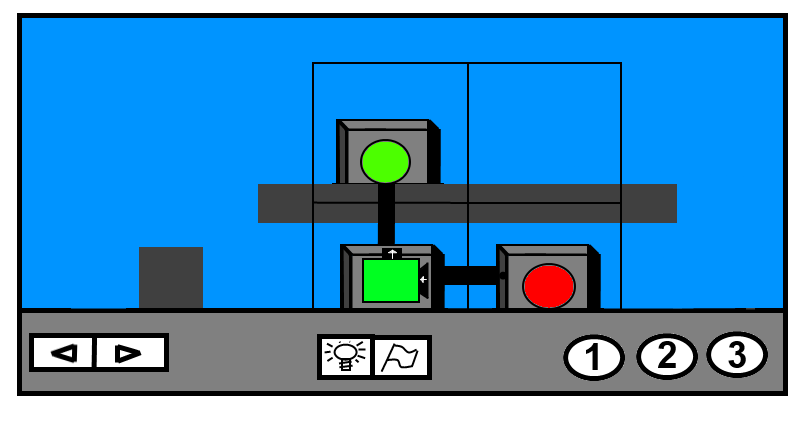
\includegraphics[scale=0.5]{assets/LevelVerarbeitungBsp}\\
			Maschine mit zwei Metallobjekten gleicher Farbe in darüberlegender Verschachtelungsebene.\\
			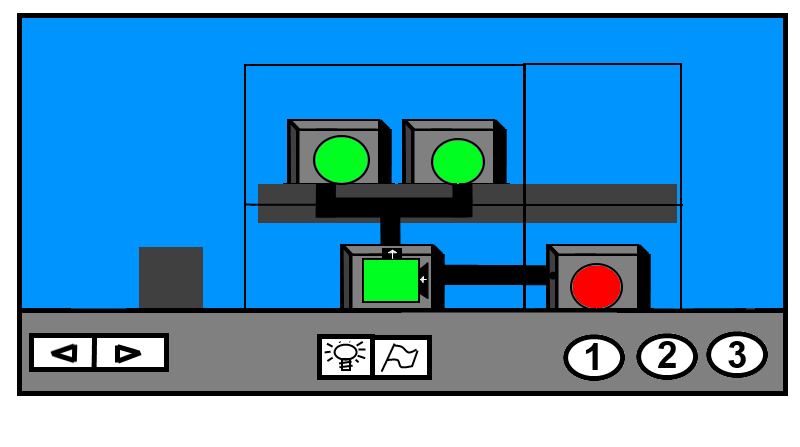
\includegraphics[scale=0.5]{assets/LevelBsp2Out}\\
		\end{minipage}
		
		\begin{minipage}{1\textwidth}
			Maschine mit einem Metallobjekt gleicher Farbe und einem Metallobjekt anderer Farbe in darüberlegender Verschachtelungsebene.\\
			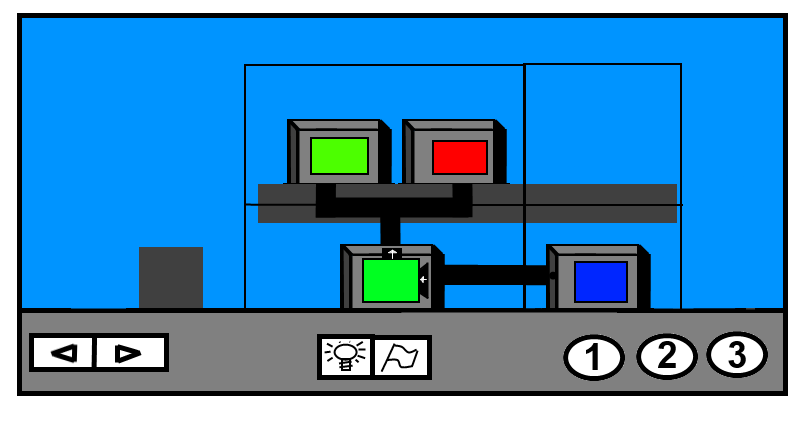
\includegraphics[scale=0.5]{assets/LevelBsp2Out1OC}\\
		\end{minipage}

	\item[Auswertungsbeispiele:] \label{Levelaufbau:Auswertungsbeispiele} Hier sehen Sie ein Beispiel für den Ablauf einer Auswertung sowie Beispiele für einige andere Auswertungen.\\
	
		\begin{minipage}{1\textwidth}
			Start der Auswertung eines Konstrukts, bestehend aus einer grünen Maschine mit einem zugehörigen Output-Metallobjekt und einem roten Metallobjekt rechts daneben.\\ 
			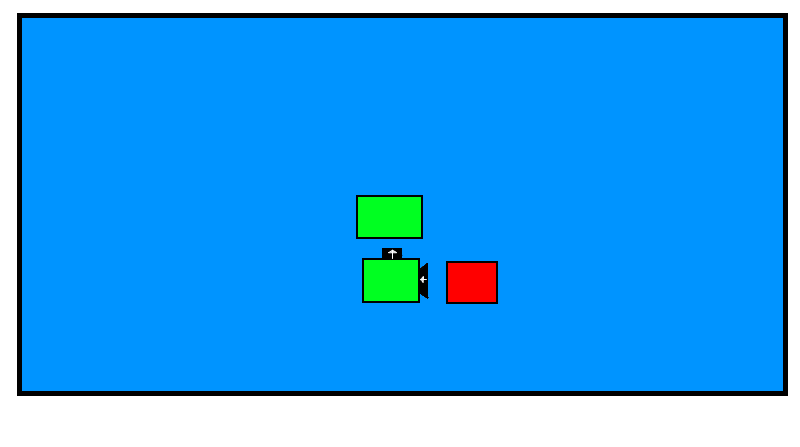
\includegraphics[scale=0.5]{assets/AuswertungAnimPic1}
		\end{minipage}
		
		\begin{minipage}{1\textwidth}
			Zuerst zieht die Maschine das Input-Objekt zur Analyse ein.\\ 
			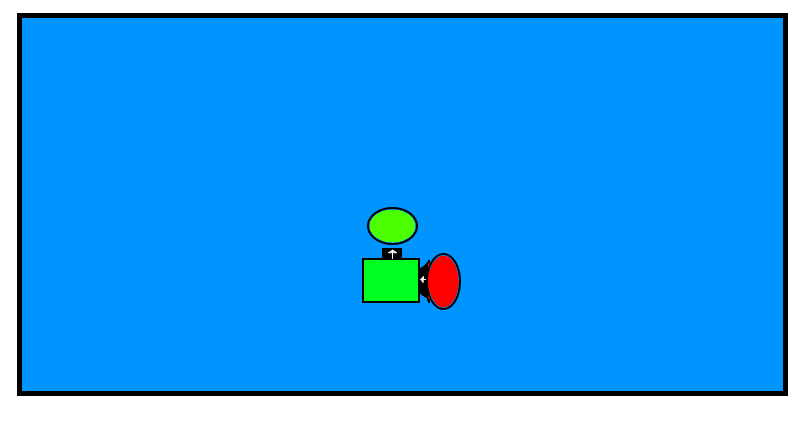
\includegraphics[scale=0.5]{assets/AuswertungAnimPic2}
		\end{minipage}
		
		\begin{minipage}{1\textwidth}
			Nach Beendigung des Einlesevorgangs beginnt die Maschine mit der Verarbeitung der Output-Objekte.\\ 
			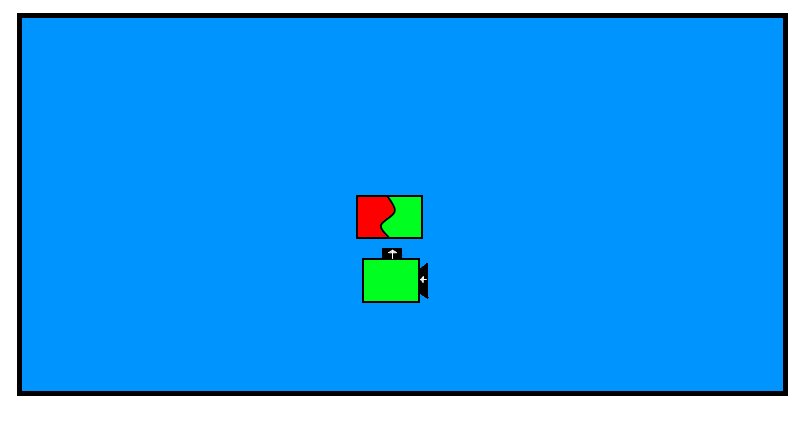
\includegraphics[scale=0.5]{assets/AuswertungAnimPic3}
		\end{minipage}
		
		\begin{minipage}{1\textwidth}
			Ist die Bearbeitung abgeschlossen, verschwindet die Maschine (ist kaputt) und übrig bleibt das bearbeitete Metallobjekt.\\ 
			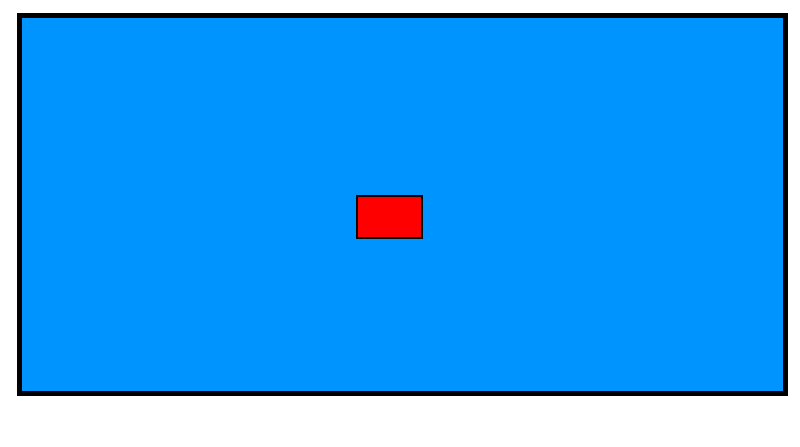
\includegraphics[scale=0.5]{assets/AuswertungAnimPic5}
		\end{minipage}
		
			Nun gilt bei der Auswertung noch zu beachten wie ein Ampel-Konstrukt arbeitet.\\
			
		\begin{minipage}{1\textwidth}
			Ist ein Ampel-Konstrukt an der Reihe zu arbeiten, so gibt es zwei Möglichkeiten:\\
			Die Ampel ist rot, was bedeutet, dass in der darüber liegenden Verschachtelung mindestens zwei Maschinen vorhanden sind. Das heißt, der normale Auswertungsablauf hält und die Verschachtelung oberhalb der roten Ampel wird ausgewertet, bis nur noch eine Maschine darin vorhanden ist. Dann schaltet die Ampel auf grün um und verschwindet anschließend. Die darüber liegende Verschachtelung rutscht um eine Ebene nach unten und setzt die normale Verarbeitung fort.\\ 
			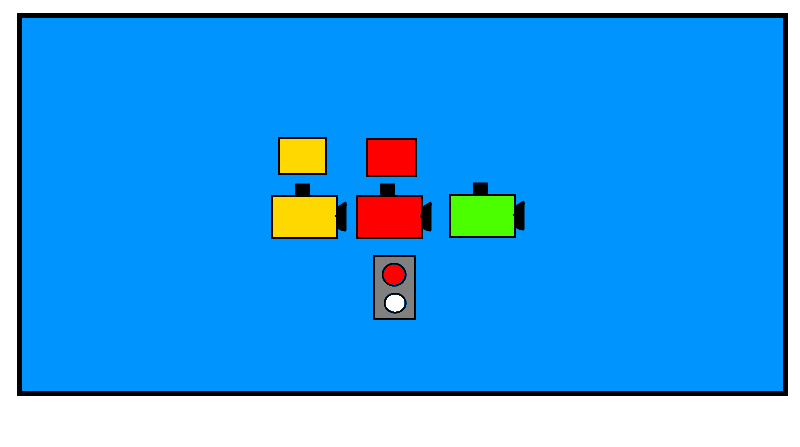
\includegraphics[scale=0.5]{assets/AuswertungAmpelRot}
		\end{minipage}
		
		\begin{minipage}{1\textwidth}
			Ist die Ampel grün, so heißt das, dass nur eine Maschine oder weniger in der darüber liegenden Verschachtelung ist. Die Ampel verschwindet und die darüber liegende Verschachtlung rutscht um eine Ebene nach unten und setzt die normale Verarbeitung fort.\\  
			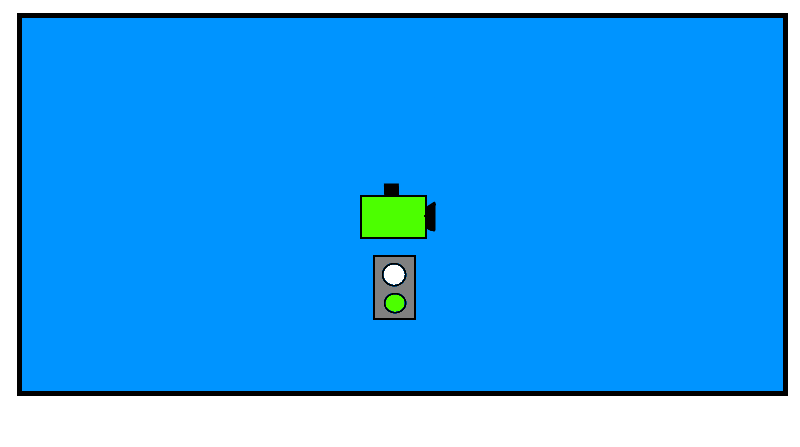
\includegraphics[scale=0.5]{assets/AsuwertungAmpelGrun}
		\end{minipage}


\end{description}

\clearpage


\subsection{Aufgabentypen} \label{subsection:Aufgabentypen}

In jedem Spieltyp läuft im Hintergrund ein Timer* mit, der die Spielzeit des Levels misst. Dadurch können Timer-\glspl{gls:achievement} * freigeschaltet werden.
\begin{enumerate}
	\item \label{aufgabentyp:puzzle} Puzzle: Aufgabentyp, bei dem an die vorgegebenen Stellen Maschinen, Metallobjekte oder Maschinen-Cluster eingefügt werden müssen, um einen $\lambda$-Ausdruck zu bauen, der ein gewünschtes Ergebnis liefert oder einen gewünschten Endzustand hat.\\
	Die benötigten Teile sind in der Spielwelt verstreut und müssen an den passenden Stellen eingefügt werden.\\
	Der \gls{gls:anwender} kann dabei immer nur ein Objekt tragen.\\
	Es sind auch falsche Konstellationen möglich, die zu einem falschen Ergebnis führen.\\
	\item \label{aufgabentyp:fehlerfindung} Fehlerfindung*: Aufgabentyp, bei dem der $\lambda$-Ausdruck schon fertig zusammengesetzt ist, jedoch nicht in der richtigen Konstellation.\\
	Der \gls{gls:anwender} muss die Fehler finden und die entsprechenden Objekte austauschen.\\
	\item \label{aufgabentyp:ergebnis} Ergebnisbestimmung*: Die Maschinenkonstruktion ist gegeben, der \gls{gls:anwender} muss mit einer gegebenen Menge an Elementen die Endkonstellation bestimmen und angeben. ($\beta$ - Reduktion durchführen) 
\end{enumerate}

\clearpage







% ---------------
% Produkteinsatz Anforderungen
% ---------------


\section{Produkteinsatz}

Das Produkt soll auf jedem \gls{gls:android}-Gerät ab \gls{gls:android} 4.2 einsatzfähig sein. Ein Einsatz auf Emulatoren der \gls{gls:android}-Plattform ist ebenfalls vorgesehen.

\subsection{Anwendungsbereich}

\begin{enumerate}
	\item Freizeitgestaltung von Kindern ab 8 Jahren
	\item Einsatz an Vor- und Grundschulen im Rahmen von Unterrichtsprojekten
\end{enumerate}

\subsection{Zielgruppen}

Die Zielgruppe besteht überwiegend aus Kindern im Alter von acht bis zwölf Jahren, die das Spiel entweder aus Interesse oder im Rahmen eines Projektes an der Schule spielen. Hierbei wird ihnen subtil der Umgang mit dem $\lambda$-Kalkül beigebracht.

\clearpage







% --------------
% Produktumgebung
% ---------------

\section{Produktumgebung}

\subsection{\gls{gls:software}}

\begin{itemize}
	\item Die \gls{gls:software} ist für die Unterstützung der API 17+ (Android 4.2) von \gls{gls:android} ausgelegt.
\end{itemize}

\subsection{\gls{gls:hardware}}

\begin{itemize}
	\item Die eingesetzte \gls{gls:hardware} muss über ein \gls{gls:touchinterface} verfügen.
	\item Das Spiel ist für die Verwendung mit einem \gls{gls:tabletcomputer} ausgelegt.
	\item Eine Verwendung mit einem \gls{gls:smartphone} soll jedoch auch möglich sein.
\end{itemize}

\clearpage








% ---------------
% Funktionale Anforderungen
% ---------------

\section{Funktionale Anforderungen}


\subsection{Tutorial} % (fold)
\label{sub:fa:tutorial}

% subsection fa:tutorial (end)

\begin{falist}
	\item \label{fa:tutorial} \textbf{Tutorial-Modus} findet nach dem ersten Starten des Spiels statt (Musskriterium \ref{muss:tutorial}).
	\begin{falist} 
        \item \label{fa:tutorial_01}Der Tutorial-Modus basiert auf einem Minimum an textuellen Erklärungen.
        \item \label{fa:tutorial_02}Erklärt die Funktionsweise des Spiels,
		\item \label{fa:tutorial_03}Ein wiederholtes Starten des Tutorial-Modus ist möglich.
	\end{falist}
\end{falist}

\subsection{\glspl{gls:benutzerprofil}}
\begin{falist}[resume]
	\item \label{fa:spielerprofile} \textbf{Spielerprofile}
	\begin{falist}
		\item \label{fa:spielerprofile_anlegen} \textbf{Anlegen von Spielerprofilen} Spielerprofile können einzeln hinzugefügt werden.
		\item \label{fa:spielerprofile_bearbeiten} \textbf{Bearbeiten von Spielerprofilen} Spielerprofile können bearbeitet werden. Das Ändern des Namens sowie der Spielfigur sind möglich.
		\item \label{fa:spielerprofile_loeschen} \textbf{Löschen von Spielerprofilen} Das Löschen eines Spielerprofils erfolgt über das Profilmneü.
		\item \label{fa:spielerprofile_wechseln} \textbf{Wechseln zu Spielerprofilen} Das Wechseln eines Spielerprofils ist möglich über das Profilmenü.
		\item \label{fa:spielerprofile_separiert} \textbf{Eigenständigkeit von Spielerprofilen} Spielerprofile sind eigenständig. Fortschritte, die in einem Spielerprofil gemacht wurden, sind an dieses \gls{gls:benutzerprofil} gebunden.
	\end{falist}
\end{falist}

\subsection{Spieldesign}

\begin{falist}[resume]
	\item \label{fa:level} \textbf{Level} Ein \gls{gls:level} hat eine Aufgabe mit gegebenem Ziel und einer Menge an Spielobjekten, die der \gls{gls:anwender} an vorgegebenen Stellen platzieren muss.
	\item \label{fa:levelmenue} \textbf{Level-Menü} bietet eine Übersicht über alle \gls{gls:level} des Spiels (Musskriterium \ref{muss:5indilevel}). Diese sind unterteilt in abgeschlossene und nicht abgeschlossene Level.
    \begin{falist}
        \item \textbf{Erstes Level} Das erste \gls{gls:level} ist automatisch freigeschaltet.
        \item \textbf{Freischalten weiterer Level} Das Freischalten weiterer Level erfolgt durch Freispielen. Beendigung eines Levels führt zum Freischalten des nächsten.
    \end{falist}
    \item \label{fa:spielen} \textbf{\gls{gls:level} spielen}
    \item \label{fa:buttons_muss} \textbf{Button / Steuerung}
    \begin{falist}
    	\item \label{fa:button_rechts_kreuz} \textbf{Drücken der rechten Pfeiltaste} Bewegt die Spielfigur in der Spielwelt nach rechts.
    	\item \label{fa:button_links_kreuz} \textbf{Drücken der linken Pfeiltaste} Bewegt die Spielfigur in der Spielwelt nach links.
    	\item \label{fa:button_lampe} \textbf{Drücken des Hinweis-Buttons} Zeigt einen neuen Dialog an, der dem Spieler einen Ausblick auf die Lösung des Levels bietet.
    	\item \label{fa:button_flagge} \textbf{Drücken des Flaggen-Buttons} Zeigt einen Dialog, der die Zielkonstellation des Levels enthält.
    	\item \label{fa:button_aufnehmen_ablegen} \textbf{Drücken des Aufnahme-/Ablegen-Buttons} Wenn die Spielfigur keine Maschine trägt, nimmt Sie die Maschine, die sich vor der Spielfigur (Blickrichtung) befindet, auf. Sollte dort keine Maschine sein, wird keine Handlung ausgeführt. Analog für das Ablegen einer Maschine.
    	\item \label{fa:button_jump} \textbf{Drücken des Sprungbuttons} Durch das Drücken des Sprungbuttons springt die Spielfigur. In Kombination mit \ref{fa:button_rechts_kreuz} und \ref{fa:button_links_kreuz} kann ein Sprung in die entsprechende Richtung erfolgen.
    	\item \label{fa:button_ducken} \textbf{Drücken des Ducken-Buttons} Durch das Drücken des Ducken-Buttons wird die Größe der Spielfigur verringert. Sobald der \gls{gls:anwender} den Button loslässt, kehrt die Figur zu ihrer ursprünglichen Größe zurück.
    \end{falist}
    \item \label{fa:button_wunsch} \textbf{Button / Steuerung *}
    \begin{falist}
    	\item \label{fa:wunsch_button_rechts} \textbf{Wischgeste nach rechts} Der \gls{gls:anwender} wischt mit seinem Finger über den Bildschirm nach rechts. Dadurch bewegt sich die Spielfigur um einen Schritt nach rechts.
    	\item \label{fa:wunsch_button_links} \textbf{Wischgeste nach links} Der \gls{gls:anwender} wischt mit seinem Finger über den Bildschirm nach links. Dadurch bewegt sich die Spielfigur um einen Schritt nach links.
    	\item \label{fa:wunsch_button_oben} \textbf{Wischgeste nach oben} Der \gls{gls:anwender} wischt mit seinem Finger über den Bildschirm nach oben. Dadurch führt die Spielfigur einen Sprung aus. Diese funktionale Anforderung ist kombinierbar mit \ref{fa:wunsch_button_rechts} und \ref{fa:wunsch_button_links}. Sollte die Spielfigur geduckt sein, richtet sie sich wieder auf.
    	\item \label{fa:wunsch_button_unten} \textbf{Wischgeste nach unten} Der \gls{gls:anwender} wischt mit seinem Finger über den Bildschirm nach unten. Dadurch beginnt die Spielfigur sich zu ducken. Sie verharrt in diesem \enquote{Modus} bis der Benutzer \ref{fa:wunsch_button_oben} ausführt.
    \end{falist}
	\item \textbf{Interaktion mit den Spielelementen aus Nr. \ref{elemente:collectable}} Sammelgegenstände, die abgelegt sind, können nicht durch den \gls{gls:anwender} passiert werden und müssen übersprungen werden (siehe \ref{fa:button_jump} bzw. \ref{fa:wunsch_button_oben}).
	\item \textbf{Interaktion mit den Boxen} Die Boxen sind in einer weiteren Ebene und können von der Spielfigur zur Ablage der Metallstücke und Maschinen benutzt werden.
	\item \label{fa:auswertung_animiert} \textbf{Animierte Auswertung der Maschinenkonstellation} Durch eine Animation wird gezeigt, wie die Verarbeitung der Maschinen stattfindet (Auswertungsbeispiel siehe \ref{Levelaufbau:Auswertungsbeispiele}).
\end{falist}

\subsection{Achievements*}

\begin{falist}[resume]
    \item \label{fa:achievements} \textbf{Achievements} sind Ziele, die von dem Spiel vorgegeben werden und gutes Spielen des \gls{gls:anwender}s auszeichnen. Angedacht dafür sind folgende:
    \begin{itemize}
    	\item Abschließen des Tutorial-Modus
    	\item Abschließen eines Kapitels
    	\item Spielzeit unterhalb einer gegebenen Schranke
    	\item Spielzeit oberhalb einer gegebenen Schranke
    	\item Fun-Achievements (Nichtschwimmer, Nachtschwärmer)
    	\item First-Try
    \end{itemize}
\end{falist}

\subsection{Ladeverhalten}

\begin{falist}[resume]
	\item \label{fa:tipps} \textbf{Anzeigen von Tipps} Während das Spiel ein \gls{gls:level} (\ref{fa:level}) lädt, werden Tipps angezeigt.
\end{falist}

\subsection{Sonstiges}

\begin{falist}[resume]
	\item \label{fa:infobereich} \textbf{Infobereich} Das Spiel verfügt über einen Infobereich, der weiterführende Informationen zum Thema $\lambda$-Kalkül enthält.
	\item \label{fa:spieleinstellungen} \textbf{Spieleinstellungen} Das Spiel verfügt über Einstellungen, die das Verhalten des Programms beeinflussen. \ref{produktdaten:einstellungen}
	\item \label{fa:spielestatistiken} \textbf{Spielstatistiken} Das Spiel verfügt über Spielstatistiken, die über das Verhalten des Spielers Auskunft geben. \ref{produktdaten:spielestatistiken}
	
\end{falist}

\clearpage








% ---------------
% Produktdaten
% ---------------

\section{Produktdaten}
Das Produkt speichert und verwaltet Daten, insbesondere: 

\subsection{Profildaten}

\begin{pdlist}
    \item \label{produktdaten:profile} \glspl{gls:benutzerprofil}, bestehend aus 
    \begin{pdlist}
        \item \label{produktdaten:profile:name}Name des Spielers
        \item \label{produktdaten:profile:avatar}Avatar
        \item \label{produktdaten:profile:einstellungen}profilbezogene Einstellungen (Hintergrund, Musik etc.) 
        \item \label{produktdaten:profile:spielfortschritt}profilbezogener Spielfortschritt(gelöste Level, Achievements etc.)
    \end{pdlist}
\end{pdlist}

\subsection{Spielstatistiken}
\label{produktdaten:spielestatistiken}

\begin{pdlist}[resume]
    \item Spieldauer
    \item Anzahl gelöste Level
    \item Anzahl Achievements*
\end{pdlist}

\subsection{Einstellungen}
\label{produktdaten:einstellungen}

\begin{pdlist}[resume]
	\item Einstellen der Lautstärke
	\item Rechts- oder Linkshänder-Modus*
\end{pdlist}

\clearpage








% ---------------
% Nichtfunktionale Anforderungen
% ---------------

\section{Nichtfunktionale Anforderungen}

\subsection{Allgemeine Ziele}

\begin{nflist}
    \item Die Navigation durch das Spiel ist für den \gls{gls:anwender} intuitiv, unabhängig von seinem Alter.
    \item Das Spiel ist insgesamt kindgerecht entworfen, d.h.:
    \begin{itemize}
    \item Weitestgehend werden Piktogramme verwendet.
    \item Textuelle Erklärung (insbesondere das $\lambda$-Symbol) wird nach Möglichkeit vermieden. Falls Text nötig ist, wird einfache, kindgerechte Sprache verwendet.
    \end{itemize}
\end{nflist}

\subsection{Benutzbarkeit, Performance, Stabilität}
\begin{nflist}[resume]
	\item Das Starten eines Levels beträgt höchstens 10 Sekunden. 
	\item Das Programm läuft stabil: 
	\begin{nflist}
		\item Es tritt kein Fehlverhalten der \gls{gls:software} auf.
		\item Ladezeiten befinden sich in einem akzeptablen Rahmen. 
	\end{nflist}
	\item Die Auswertung eines Levels(Sieg oder Niederlage) dauert max. 5 Sekunden.
	\item Der benötigte Speicherverbrauch reduziert sich auf ein Minimum. 
	\item Nach Beendigung eines Levels wird der Spielstand automatisch gespeichert.
	\item Die maximale Anzahl an Spielerprofilen ist auf 5 begrenzt.
\end{nflist}

\subsection{Qualität und Rechtliches}

\begin{nflist}[resume]
	\item Die bei diesem Projekt entstehenden Daten haben folgende Eigenschaften:
	\begin{itemize}
		\item leicht zu warten
		\item dokumentiert (\gls{gls:javadoc})
		\item getestet (\gls{gls:eclemma}, \gls{gls:junit})
		\item erweiterbar
	\end{itemize}
	\item Das Programm verwendet für Dateien folgende Standards: 
	\begin{itemize}
		\item WAV, OGG, MP3 für Audio Dateien 
		\item SVG für Vektorgrafiken
		\item PNG, JPG für pixelbasierte Grafiken
		\item JSON, XML für strukturierte Textdateien
	\end{itemize}
	\item Die Auslieferung der finalen Version erfolgt in Form einer .apk-Datei.
	\item Es wird nur ein Minimum an Berechtigungen eingefordert. Diese sind Lese- und Schreibzugriff.
\end{nflist}

\clearpage







% -------------------------
% Globale Testfälle
%-------------------------

\section{Globale Testfälle}

\subsection{Funktionssequenzen}

\begin{telist}
	\item{Erstes Ausführen des Spiels} \label{szenarien:first_run}
	\begin{itemize}
		\item Starten der Applikation durch Anklicken der App-Verknüpfung
		\item Der Ladebildschirm(\ref{appaufbau:Ladebildschirm}) wird sichtbar und informiert über den Ladezustand des Spiels.
		\item Der \gls{gls:anwender} wird direkt zum "`Benutzer-Anlegen"'- Bereich weitergeleitet
		\item Wurde ein \gls{gls:benutzerprofil} angelegt, öffnen sich die Einstellungen
		\item Geht der \gls{gls:anwender} von den Einstellungen weiter, beginnt der Tutorial-Modus
		\item Lambdalino begrüßt den \gls{gls:anwender}
		\item Es wird in die Handlung des Spiels eingeführt
		\item Nach dem Tutorial-Modus öffnet sich das Level-Menü und das erste \gls{gls:level} ist freigeschaltet 
	\end{itemize}
	
	\item{Allgemeiner Spielstart} \label{szenarien:allg_spielstart}
	\begin{itemize}
		\item Starten der Applikation durch Anklicken der App-Verknüpfung
		\item Der Ladebildschirm(\ref{appaufbau:Ladebildschirm}) wird sichtbar und informiert über den Ladezustand des Spiels
		\item Nach dem Laden kann man den Benutzer aus vorhandenen Profilen auswählen oder man legt ein neues \gls{gls:benutzerprofil} an
		\item Das Hauptmenü (\ref{appaufbau:Hauptmenü}) wird geöffnet		
	\end{itemize}
	
	\item Tutorial basierend auf (\ref{fa:tutorial} - \ref{fa:tutorial_03})
	\begin{itemize}
		\item Der \gls{gls:anwender} startet den Tutorial-Modus über das Level-Menü (Systemmodell \ref{appaufbau:Levelauswahl}) oder gelangt automatisch in diesen beim ersten Starten des Spiels mit einem neuen \gls{gls:benutzerprofil}.
		\item Der \gls{gls:anwender} wird durch die Tutorial-\gls{gls:level} geleitet, in denen ihm erklärt wird, wie er die Steuerung benutzen muss, die Elemente in die gewünschte Ablage bringen kann und wie genau die Maschinen die Elemente verarbeiten.
		\item Wenn der Tutorial-Modus beendet wurde, gelangt der \gls{gls:anwender} zum Hauptbildschirm.
	\end{itemize}

	\item Ein \gls{gls:benutzerprofil} anlegen (\ref{fa:spielerprofile_anlegen})
	\begin{itemize}
		\item Der \gls{gls:anwender} befindet sich im Hauptmenü und drückt auf den \enquote{Benutzerverwaltungsbutton}. Diese Aktion führt den \gls{gls:anwender} zum Profilmenü.
		\item Durch Wischgesten gelangt der \gls{gls:anwender} an das Ende der Liste, wo sich ein \enquote{+}-Zeichen befindet. Durch Drücken dieses Symbols wird ein neuer Dialog gestartet.
		\item In diesem Dialogfenster kann der \gls{gls:anwender} einen neuen Profilnamen angeben. Durch Drücken des \enquote{Weiter}-Buttons gelangt er zu einem weiteren Dialog.
		\item In diesem Dialog kann er einen Charakter und ob dieses \gls{gls:benutzerprofil} im Rechts- oder Linkshänder Modus* gespielt werden soll auswählen. Der Dialog wird durch Betätigen des \enquote{OK}-Buttons beendet.
	\end{itemize}
	
	\item Ein \gls{gls:benutzerprofil} auswählen (\ref{fa:spielerprofile_wechseln})
	\begin{itemize}
		\item Der \gls{gls:anwender} befindet sich im Hauptmenü und drückt auf den \enquote{Benutzerverwaltungsbutton}. Diese Aktion führt den \gls{gls:anwender} zum Profilmenü.
		\item Durch Scrollen kann der \gls{gls:anwender} seine \glspl{gls:benutzerprofil} einsehen. Bei Erreichen des gewünschten Profils wählt er dieses durch Berühren aus.
	\end{itemize}
	
	\item Ein \gls{gls:benutzerprofil} löschen (\ref{fa:spielerprofile_loeschen})
	\begin{itemize}
		\item Der \gls{gls:anwender} befindet sich im Hauptmenü und drückt auf den \enquote{Benutzerverwaltungsbutton}. Diese Aktion führt den \gls{gls:anwender} zum Profilmenü.
		\item Durch Scrollen kann der \gls{gls:anwender} seine \glspl{gls:benutzerprofil} einsehen. Er wählt diese jeweils durch Berühren aus. 
	\end{itemize}
	
	\item Ein \gls{gls:benutzerprofil} bearbeiten (\ref{fa:spielerprofile_bearbeiten}) \label{test:profilBeartbeiten}
	\begin{itemize}
		\item Der \gls{gls:anwender} befindet sich im Hauptmenü und drückt auf den \enquote{Benutzerverwaltungsbutton}. Diese Aktion führt den \gls{gls:anwender} zum Profilmenü.
		\item Der \gls{gls:anwender} wählt den \enquote{Bearbeitungs-Button} neben dem \gls{gls:benutzerprofil}, welches er bearbeiten möchte, aus.
		\item Im Bearbeitungsbereich kann der \gls{gls:anwender} seinen Namen, Avatar und die Position der Steuerung (Rechts-oder Linkshänder- Modus)*  verändern.
	\end{itemize}
	
	\item{Informationen aufrufen} \label{szenarien:infomartionen_aufrufen} (\ref{fa:infobereich})
	\begin{itemize}
		\item Im Hauptmenü wählt man den Punkt \enquote{Einstellungen}
		\item Dort klickt man auf den Button \enquote{Infos}.
		\item Es erscheint eine vereinfachte Erklärung des Lambda-Kalküls, sowie eine Erläuterung zu den Zusammenhängen des Lambda-Kalküls mit dem Spiels.
	\end{itemize}
	
	\item Level-Menü (\ref{fa:levelmenue})
	\begin{itemize}
		\item Der \gls{gls:anwender} kann nur jene \gls{gls:level} öffnen, die bereits freigeschaltet wurden. Die anderen \gls{gls:level} sind sichtbar, können jedoch nicht ausgewählt werden.
	\end{itemize}
	
	\item \gls{gls:level} spielen (\ref{fa:spielen})
	\begin{itemize}
		\item Die Figur reagiert korrekt auf die Steuerung.
		\item Die Steuerung befindet sich auf der Seite, die der \gls{gls:anwender} im \gls{gls:benutzerprofil} ausgewählt hat (\ref{test:profilBeartbeiten}).
		\item Alle Elemente, die für das Lösen des Levels benötigt werden, sind vorhanden.
		\item Alle Elemente sind für die Figur erreichbar.
		\item Die Ablagen für die Elemente sind vorhanden.
		\item Die Elemente können von der Figur aufgenommen werden.
		\item Nachdem die Elemente aufgenommen wurden, werden sie von der Figur getragen.
		\item Die Elemente können wieder abgesetzt werden.
		\item Die Elemente können in die Ablagen platziert werden.
		\item Ist im Level ein Ampel-Konstrukt vorhanden, so ist die Ampel rot solange mehr als eine Maschine oberhalb der Ampel in der Verschachtelung existieren.
		\item Ist im Level ein Ampel-Konstrukt vorhanden, so wird die Ampel grün sobald nur noch eine Maschine oder keine oberhalb der Ampel in der Verschachtelung existieren.
		\item Sind die Elemente falsch positioniert, öffnet sich die Tür nicht und die Figur muss sie umordnen, um sie richtig zu platzieren.
		\item Die Tür öffnet sich, wenn alle Elemente korrekt platziert wurden.
	\end{itemize}
	
	\item Buttons (\ref{fa:button_rechts_kreuz} - \ref{fa:button_ducken})
	\begin{itemize}
		\item Nachdem der \gls{gls:anwender} das Spiel gestartet hat, werden die Buttons, spezifiziert in den funktionalen Anforderungen, angezeigt.
		\item Alle Buttons haben die Funktionsweise, die jeweils spezifiziert wurde.
	\end{itemize}
	
	\item Spieleinstellungen (\ref{produktdaten:einstellungen})
	\begin{itemize}
		\item Der \gls{gls:anwender} kann die Lautstärke verändern. Die Hintergrundmusik wird dementsprechend lauter oder leiser.
		\item Der \gls{gls:anwender} kann wählen, ob die Musik an oder aus sein soll.
	\end{itemize}
	
	\item Spielestatistiken (\ref{produktdaten:spielestatistiken})
	\begin{itemize}
		\item Der \gls{gls:anwender} kann in den Spielestatistiken sehen, wie lange er bereits gespielt, wie viele \gls{gls:level} er gelöst und welche Achievements* er bereits erreicht hat.
	\end{itemize}
	
	\item{Spiel verlassen} \label{szenarien:quit_game}
	\begin{itemize}
		\item Spiel beenden
		\begin{enumerate}
			\item Man klickt auf den Button links oben im Hauptmenü
			\item Es erscheint ein Fenster \enquote{Wirklich verlassen?}
			\item Beim Betätigen des Button \enquote{Ja} wird das Spiel verlassen und die App beendet
			\item Außerdem werden alle nicht gespeicherten Änderungen gespeichert
		\end{enumerate}
		\item Spiel über das Betriebssystem verlassen
		\begin{enumerate}
			\item Der Benutzer berührt den Home-Button auf seinem Gerät, um zurück zu \gls{gls:android} zu gelangen.
		\end{enumerate}
	\end{itemize}
	
	\item Speichern / Laden von Applikationszuständen
	\begin{itemize}
		\item Beim Verlassen des Spiels durch Hardware-Tasten oder ähnliches begibt sich das Spiel in den Pausenmodus mit Buttons zum Neustart des Levels, dem Verlassen ins Level-Menü, dem Verlassen ins Hauptmenü und zu den Einstellungen (Lautstärke) sowie der Option, weiterzuspielen.
		\item Wenn der \gls{gls:anwender} die Anwendung erneut aufruft, findet er dieses Pause Menü vor.
	\end{itemize}
	
	\item Speichern / Laden von Spielzuständen
	\begin{itemize}
		\item Spielzustände werden automatisch vom Spiel bei Beendigung eines Levels gespeichert.
		\item Spielzustände werden beim Auswählen eines Levels geladen und sind identisch mit den gespeicherten.
	\end{itemize}
\end{telist}

\subsection{Datenkonsistenz}

\begin{telist}[resume]
	\item Der Spielfortschritt eines jeden Profils wird unabhängig von den anderen Profilen gespeichert und verwaltet. Im Spielfortschritt eingeschlossen sind die Achievements* des jeweiligen Nutzers.
	\item Das Anlegen zweier Profile, die über den selben Namen verfügen, ist nicht gestattet. Sollte der \gls{gls:anwender} sich dazu entschließen, ein \gls{gls:benutzerprofil} zu löschen, wird der Name wieder freigegeben und kann für ein neues \gls{gls:benutzerprofil} verwendet werden.
\end{telist}

\clearpage











% ---------------
% Systemmodelle
% ---------------
\section{Systemmodelle}

\subsection{Allgemeine Appaufteilung}

Der hier gezeigte Systemaufbau ist lediglich eine grobe \enquote{Skizze},
die die Zusammenhänge zwischen den einzelnen Menüs, sowie
die Gestaltung und Aufteilung der App verdeutlichen soll.\\
Allgemein gilt jedoch, dass so viel wie möglich ohne Text, sondern durch Symbolik erklärt bzw. dargestellt werden soll, da die Zielgruppe nicht zwangsläufig lesen und schreiben kann.\\

\begin{enumerate}
	\begin{minipage}{1\textwidth}
		\item \subsection*{Ladebildschirm:} \label{appaufbau:Ladebildschirm}
		Nach dem Starten der App öffnet diese im Ladebildschirm. Hier werden für die App notwendige Daten geladen, um zu garantieren, dass das Spiel flüssig und fehlerfrei läuft. Benutzereingaben sind zu diesem Zeitpunkt nicht möglich.\\
		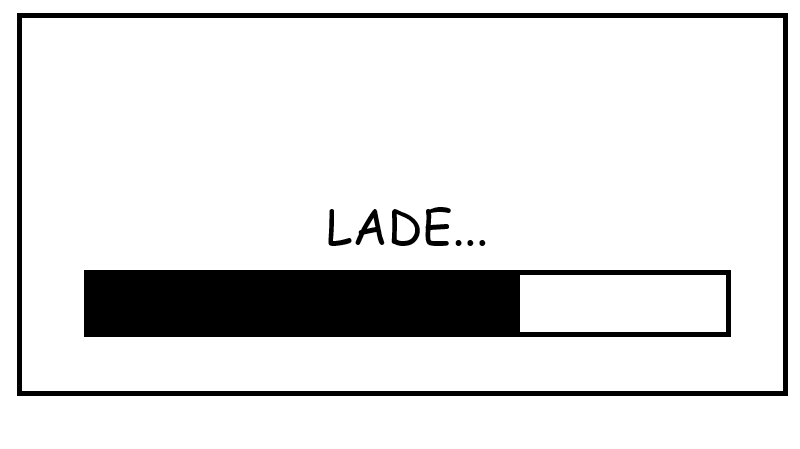
\includegraphics[scale=0.5]{assets/LoadScreen}
	\end{minipage}
	
	\begin{minipage}{1\textwidth}
		
		\item \subsection*{Profilmenü:} \label{appaufbau:Profilmenue}
		Das Profilmenü öffnet sich unmittelbar nach erfolgreicher Beendigung des Ladevorgangs (nähere Informationen zum Ablauf und Ausnahmen folgen im Kapitel Szenarien) und kann jederzeit über den \enquote{Benutzerverwaltungsbutton} im Hauptmenü aufgerufen werden.\\
		Die einzelnen Spielerprofile werden durch Anzeige des Avatars / der Spielfigur sowie den zugehörigen Profilnamen bestimmt.\\
		Es gibt eine maximale Anzahl an Spielerprofilen, sollte diese erreicht sein, so verschwindet der Button zum Erzeugen eines neuen Profils.\\
		Gleichzeitig muss immer mindestens ein Spielerprofil vorhanden sein. Sollte es nur noch ein Spielerprofil geben, so kann dieses nicht gelöscht werden, bis ein weiteres Profil angelegt wurde.\\
		In diesem Menü kann der Spieler aus den bestehenden Spielerprofilen auswählen oder in das Menü zum Anlegen eines neuen Spielers gelangen.\\
		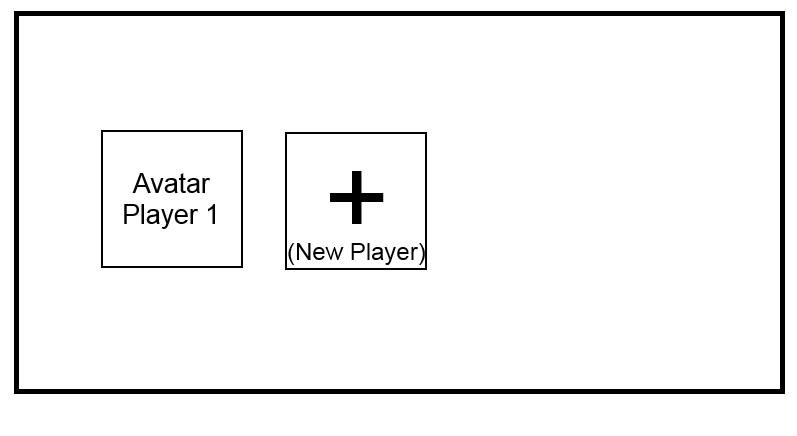
\includegraphics[scale=0.5]{assets/PlayerScreen}
	\end{minipage}
	
	\begin{minipage}{1\textwidth}
		\item \subsection*{\gls{gls:benutzerprofil} anlegen:}
		In diesem Menü kann ein neues Spielerprofil vom Spieler angelegt werden.\\
		Der Spieler kann einen Namen für das \gls{gls:benutzerprofil} eingeben und aus einer gegebenen Menge an Avataren bzw. Avatarteilen einen als Identifikationsmerkmal aussuchen beziehungsweise zusammensetzen.\\
		Der gewählte Avatar dient im weiteren Verlauf auch als Spielfigur, wobei jedoch bis auf das Aussehen keine Unterschiede zwischen den einzelnen Figuren bestehen: Alle sind gleich groß, schnell etc.\\
		Auch die Wahl, ob man als Links- oder Rechtshänder spielen will, kann hier \gls{gls:benutzerprofil}spezifisch gewählt werden.\\
		Man kann jederzeit über das Benutzerverwaltungsmenü hierhin gelangen, um Änderungen am \gls{gls:benutzerprofil} vorzunehmen.\\
		Sollte der Spieler hier abbrechen, so gelangt er zurück ins Profilmenü. Ansonsten landet er entweder im Tutorial oder im Hauptmenü(Mehr dazu im Kapitel Szenarien)\\
		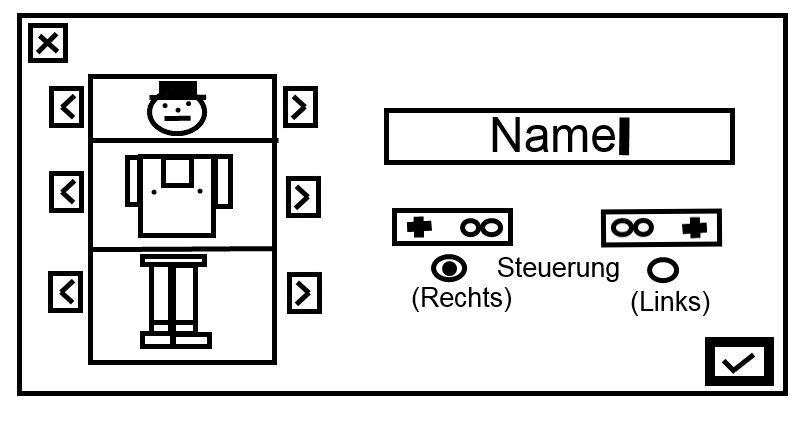
\includegraphics[scale=0.5]{assets/CreateProfile2}
	\end{minipage}
	
	\begin{minipage}{1\textwidth}
		\item \subsection*{Hauptmenü:} \label{appaufbau:Hauptmenü}
		Dies ist der zentrale Knotenpunkt der App.\\
		Von hier aus kann der Spieler zur Stageauswahl, den Einstellungen, seiner Statistik, zurück ins Profilmenü gelangen oder das Spiel komplett verlassen.\\
		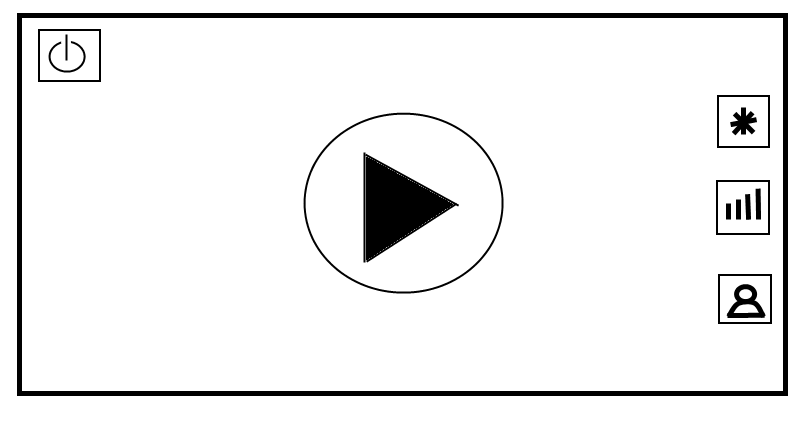
\includegraphics[scale=0.5]{assets/Mainmenu}
	\end{minipage}
	
	\begin{minipage}{1\textwidth}
		\item \subsection*{Einstellungen:}
		Hier können verschiedene grundlegende Einstellungen vorgenommen werden.\\
		Von hier gelangt man zur Ansicht aller Achievements (Achievementmenü).\\
		Der Zurück-Button führt ins Hauptmenü, beim Verlassen werden sämtliche Änderungen automatisch gespeichert.\\
		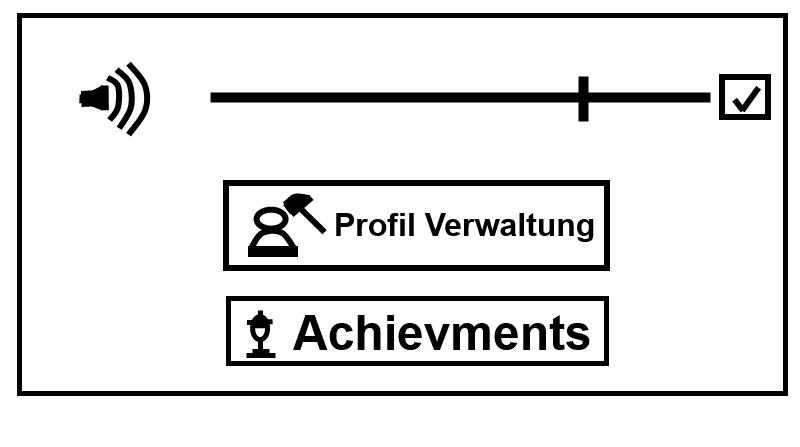
\includegraphics[scale=0.5]{assets/Einstellungen}
	\end{minipage}

	\begin{minipage}{1\textwidth}
		\item \subsection*{Profilbearbeitungsmenü:}
		Dieses Menü ist identisch mit dem Menü zum Anlegen eines neuen Spielerprofils und erreichbar über das Profilmenü.\\
		Beendet man dieses Menü, kommt man automatisch zurück ins Hauptmenü.\\
		Außerdem kann hier ein bestehendes \gls{gls:benutzerprofil} gelöscht werden. Sollte man ein \gls{gls:benutzerprofil} löschen, so landet man anschließend im Profilmenü um ein anderes \gls{gls:benutzerprofil} zu wählen.\\
		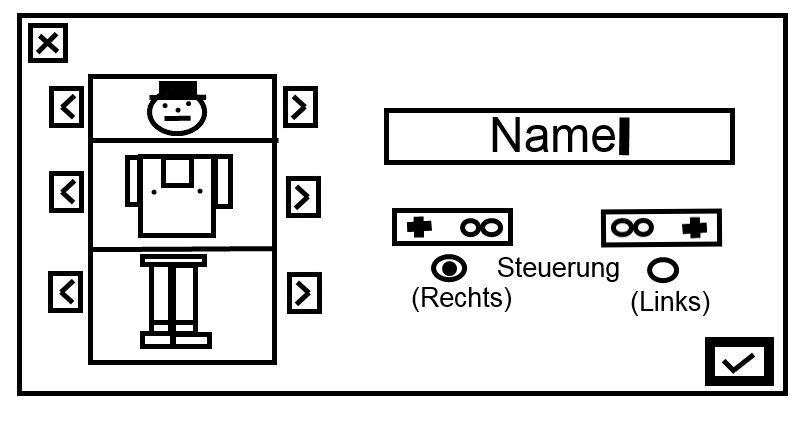
\includegraphics[scale=0.5]{assets/CreateProfile2}
	\end{minipage}

	\begin{minipage}{1\textwidth}
		\item \subsection*{Achievements:}
		Hier sind alle Achievements zu sehen. Schon erreichte sind durch ein Bild gekennzeichnet, ansonsten ist dort ein Platzhalter zu sehen. Ein Abbruch führt zurück in die Einstellungen.\\
		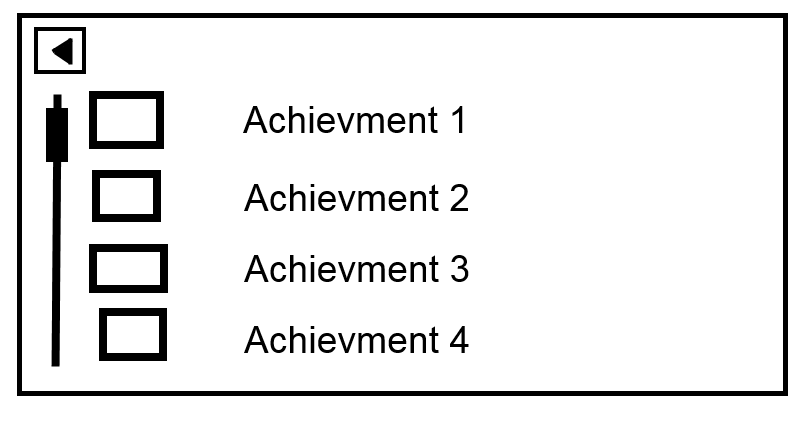
\includegraphics[scale=0.5]{assets/Achievments}
		
	\end{minipage}
	
	\begin{minipage}{1\textwidth}
		\item \subsection*{Stageauswahl:}
		Hier kann man der Anwender eine Stage zum Spielen auswählen. Sie sind der Schwierigkeit nach geordnet und können im Spielverlauf freigeschaltet werden.\\
		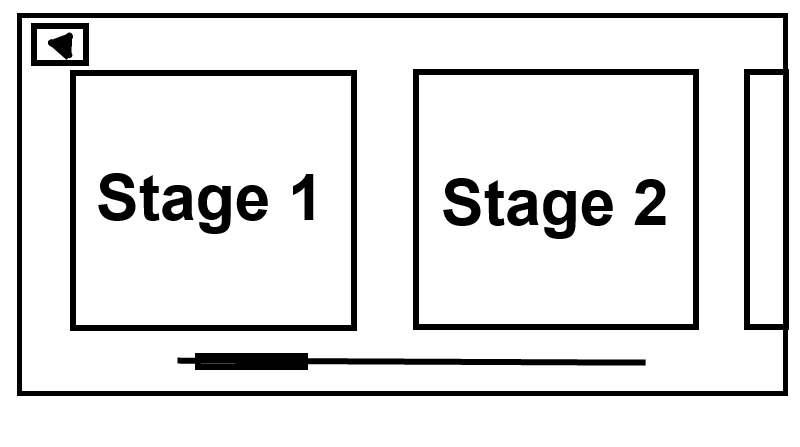
\includegraphics[scale=0.5]{assets/Stagemenu}
	\end{minipage}
	
	\begin{minipage}{1\textwidth}
		\item \subsection*{Levelauswahl:} \label{appaufbau:Levelauswahl}
		Hier kann ein \gls{gls:level} der Stage, in der man sich aktuell befindet, gestartet werden (auch diese müssen nach und nach freigeschaltet werden).\\
		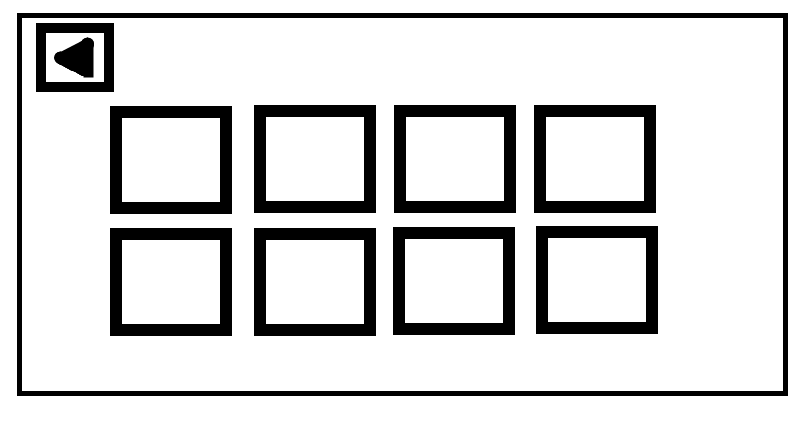
\includegraphics[scale=0.5]{assets/Levelmenu}
	\end{minipage}
	
	\begin{minipage}{1\textwidth}
		\item \subsection*{Leveldesign:} \label{appaufbau:Leveldesign}
		Jedes \gls{gls:level}  hat den selben Aufbau: Am unteren Rand sind die Buttons und das Steuerkreuz zum Bedienen der Spielfigur sowie ein Button, um sich das aktuelle Level-Ziel anzeigen oder Hinweise zum \gls{gls:level} geben zu lassen.\\ Die Anordnung der Buttons wird gespiegelt, falls man als Linkshänder spielen will. Der komplette Buttonbereich ist transparent, sodass der Spieler mehr vom Spielfeld sieht.\\
		In der linken, oberen Ecke ist ein Button, der ins Level-Menü führt. Das Spiel wird dann pausiert und es erscheinen Buttons zum Neustart des Levels, dem Verlassen ins Level-Menü, dem Verlassen ins Hauptmenü und zu den Einstellungen (Lautstärke).\\
		Das eigentliche Spielfeld nimmt den Rest des Bildschirms ein.\\
		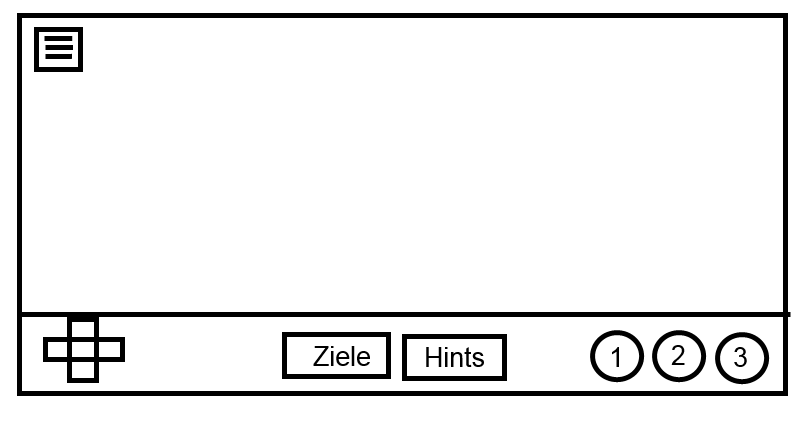
\includegraphics[scale=0.5]{assets/LevelDesign2}
	\end{minipage}
	
	\begin{minipage}{1\textwidth}
		\item \subsection*{Auswertungsmenü:}
		Sollte der Spieler ein \gls{gls:level} erfolgreich gelöst haben, so kommt er ins Auswertungsmenü. Hier werden ihm Informationen zu seinem Erfolg , sowie errungene Achievements mitgeteilt. Er hat die Wahl, das nächste \gls{gls:level} zu starten oder zurück zum Hauptmenü zu gelangen. 
		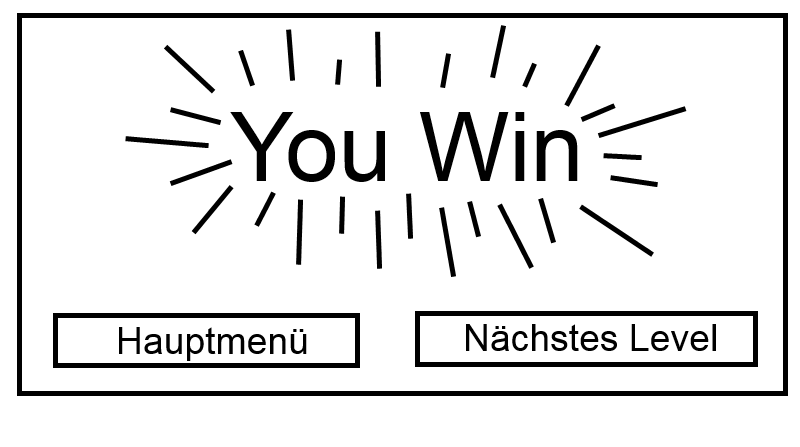
\includegraphics[scale=0.5]{assets/Auswertungsmenu}
	\end{minipage}

\end{enumerate}

\clearpage

\begin{minipage}{1\textwidth}
\subsection{Appstruktur}
	Die folgende Grafik stellt die Struktur der App grafisch dar.\\
	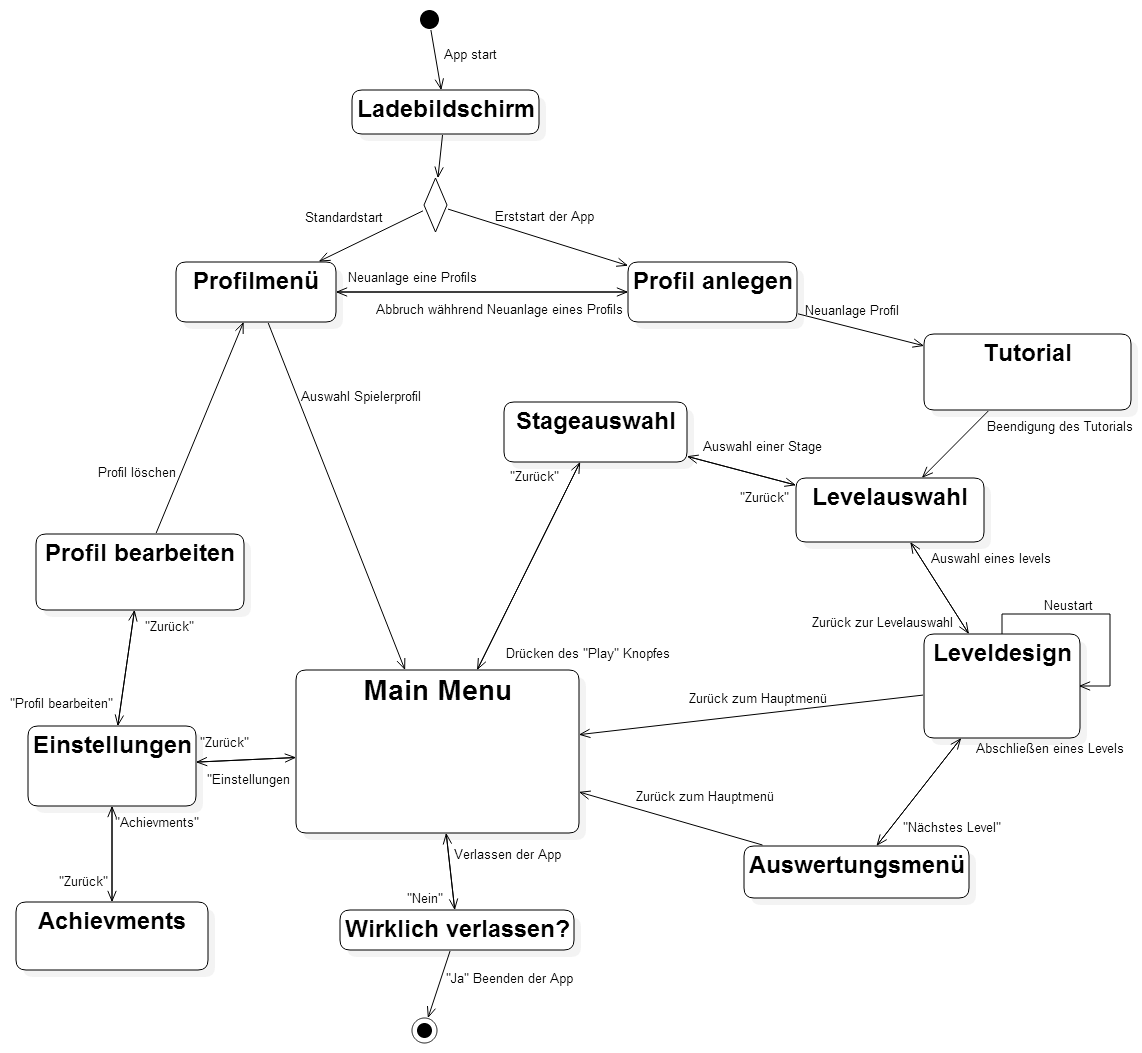
\includegraphics[width=\textwidth]{assets/Menustructur}
\end{minipage}

\begin{minipage}{1\textwidth}
\subsection{Benutzer Interaktionen}
Die folgende Grafik enthält die Möglichkeiten des Anwenders, auf die App einzuwirken.\\
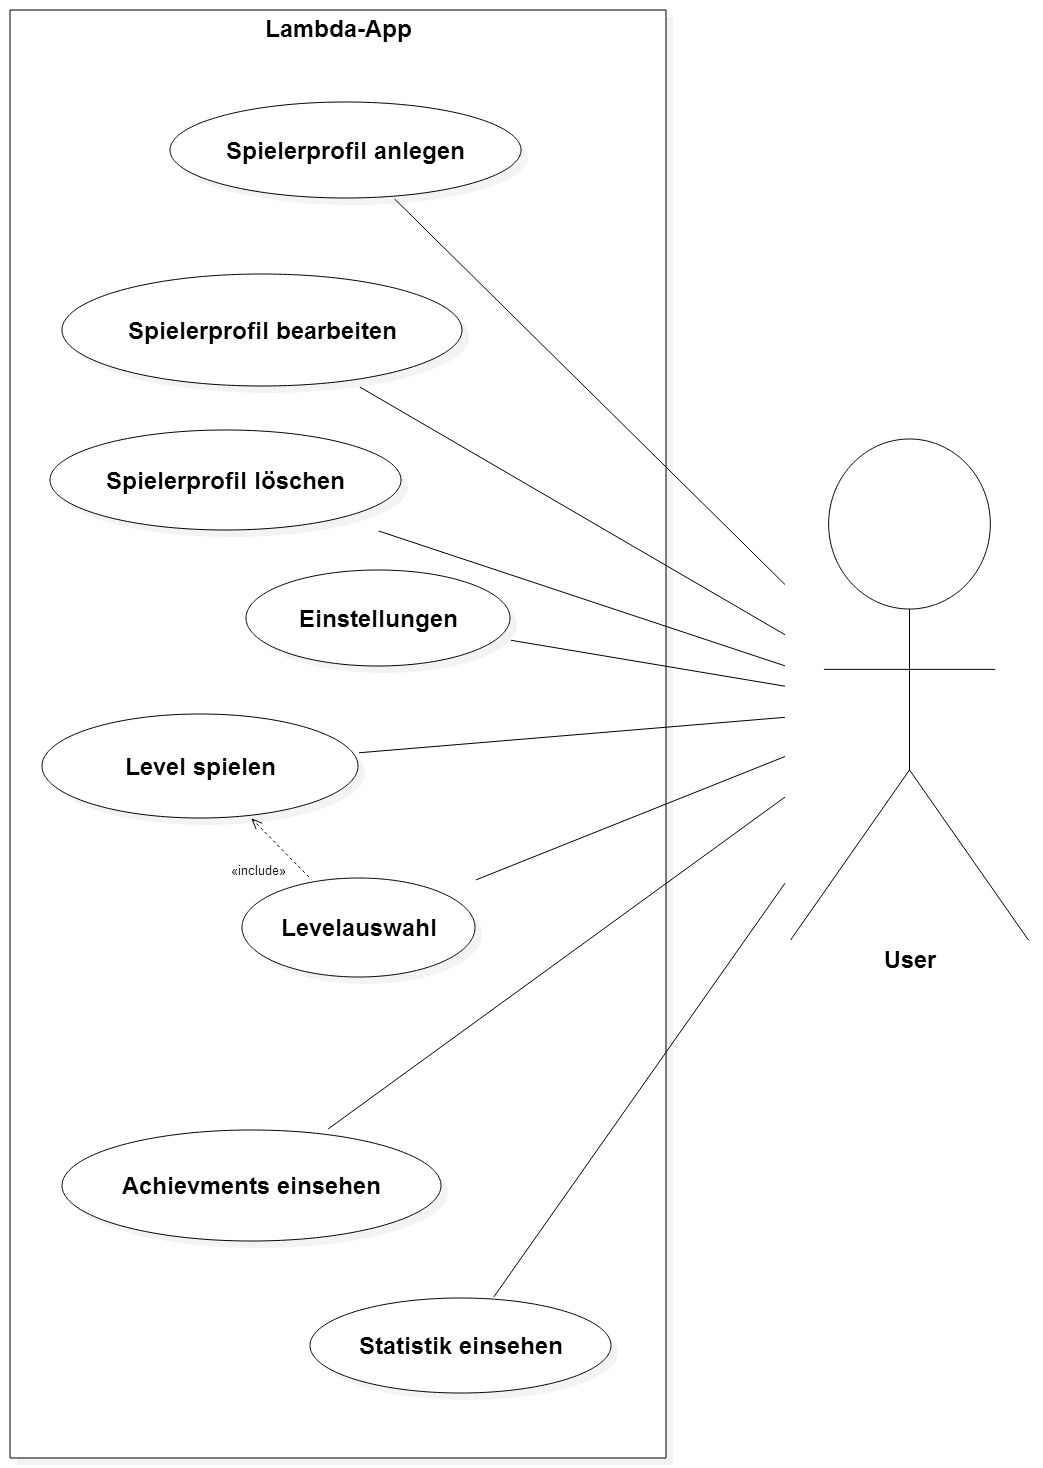
\includegraphics[width=\textwidth]{assets/Benutzerdiagramm}
\end{minipage}

\clearpage






% \glsaddall
\glossarystyle{altlist}
\printglossary[title=Glossar]
\thispagestyle{empty}
    

\end{document}